\documentclass[12pt]{report}

\linespread{1.5}

\usepackage[english,brazil]{babel}
\usepackage[letterpaper,top=2cm,bottom=2cm,left=3cm,right=3cm,marginparwidth=1.75cm]{geometry}
\usepackage[colorlinks=true, allcolors=blue]{hyperref}
\usepackage{lscape}
\usepackage{amsmath}
\usepackage{amssymb}
\usepackage{amsfonts}
\usepackage{graphicx}
\usepackage{multirow}
\usepackage{adjustbox}
\usepackage{mathtools}
\usepackage[graphicx]{realboxes}
\usepackage[table,xcdraw]{xcolor}

\title{BRAVO: Brazilian-portuguese Emotional Intensity Recognition Assistant for Voice}
\author{Brandão, H. T.}

% ==========================================================================================+
% QUALIFICAÇÃO DE MESTRADO                                                                  |
% ==========================================================================================+

\begin{document}
\maketitle

\begin{abstract}
A fala costuma ser a nossa primeira forma de comunicação e de expressão de emoções. O Reconhecimento de Emoção na Fala (Speech Emotion Recognition, SER) é um problema complexo, pois a expressão emocional depende da linguagem falada, dialeto, sotaque e histórico cultural dos indivíduos. Além disso, a intensidade dessa emoção pode afetar nossa percepção das emoções e nos induzir a interpretar a informação de forma inadequada. Embora sejam encontrados trabalhos de speech-to-text que investigam a intensidade das emoções, ao pesquisar o atual estado da arte, percebemos a escassez de trabalhos envolvendo SER e o idioma portugues. Mesmo com perspectivas de aplicabilidade em diversas áreas como monitoramento de pacientes, segurança, sistemas comerciais e entretenimento, parece haver uma ausência de trabalhos abordando a classificação da intensidade da emoção em português. Independente de formação enquanto profissionais de saúde mental, é natural que consigamos atribuir alguma espécie de métrica para comparar duas instâncias de uma mesma emoção que tenhamos sentido. Parece trivial quando atestamos que, entre dois momentos experimentando uma mesma emoção, um foi mais ou menos intenso do que o outro, ou até que ambos tiveram a mesma intensidade. Portanto, somos capazes de identificar emoções, quantificar sua intensidade e calcular uma distância para poder efetuar essa comparação. Conforme visto, trabalhos de \textit{ML} aplicados ao reconhecimento de emoções na fala vêm sendo publicados - ao menos - desde o início da década de 90 (1990), e se tornam menos frequentes quando buscamos por tarefas mais especializadas. Não tendo encontrado ocorrência na literatura, este trabalho se propõe a responder a seguinte pergunta: É possível realizar uma tarefa de aprendizado de máquina para inferir a intensidade das emoções na voz em português?\\

\noindent \textbf{Palavras-chave:} Deep Learning, SER, Intensity, brazilian portuguese, VERBO, VIVAE
\end{abstract}
\clearpage

\selectlanguage{english}
\begin{abstract}
Speech is usually our first form of communication and expression of emotions. Speech Emotion Recognition (SER) is a complex problem as emotional expression depends on the spoken language, dialect, accent and cultural background of individuals. In addition, the intensity of this emotion can affect our perception of emotions and lead us to interpret information inappropriately. Although there are speech-to-text works that investigate the emotional intensity, researching the current state of the art, we noticed the scarcity of works involving SER and the Portuguese language. Even with perspectives of applicability in several areas such as patient monitoring, security, commercial systems and entertainment, there seems to be a lack of studies addressing the classification of emotion intensity in Portuguese. Regardless of training as mental health professionals, it is natural that we are able to assign some kind of metric to compare two instances of the same emotion that we have felt. It seems trivial when we attest that, between two moments experiencing the same emotion, one was more or less intense than the other, or even that both had the same intensity. Therefore, we are able to identify emotions, quantify their intensity and calculate a distance to be able to make this comparison. As seen, works on \textit{ML} applied to the recognition of emotions in speech have been published - at least - since the beginning of the 90's (1990), and became less frequent when we look for more specialized tasks. Having not found occurrences in the literature, this work proposes to answer the following question: Is it possible to perform a machine learning task to infer the intensity of emotions in the brazilian Portuguese?\\

\noindent \textbf{Keywords:} Deep Learning, SER, Intensity, brazilian portuguese, VERBO, VIVAE
\end{abstract}
\selectlanguage{brazil}

% ==========================================================================================

\phantomsection
\addcontentsline{toc}{chapter}{Sumário}
\tableofcontents

\phantomsection
\addcontentsline{toc}{chapter}{Lista de figuras}
\listoffigures

\phantomsection
\addcontentsline{toc}{chapter}{Lista de Tabelas}
\listoftables

\pagestyle{empty}
\pagenumbering{arabic}

% ==========================================================================================

\chapter{Projeto de Pesquisa}\label{Cap:Projeto de Pesquisa}

%  https://bdm.unb.br/bitstream/10483/27583/1/2020_GabrielCampos_LucasMoutinho_tcc.pdf

Neste capítulo é apresentada a proposta contida neste trabalho. O capítulo irá se desdobrar a partir do problema encontrado e proporá uma solução para sua realização. Adiante, irá expor a sua implementação em detalhes, tratando conhecimentos mais específicos que não estejam elucidados ao longo dos capítulos anteriores e conjecturando sobre possíveis aplicabilidades deste trabalho em áreas diversas. Finalmente, as atividades propostas para este projeto de pesquisa, juntamente com um cronograma de acompanhamento, de acordo com o estabelecido pelo Programa de Pós-Graduação em Informática da Universidade de Brasília (PPGI/UnB) para a obtenção do título de Mestre.\\

% ==========================================================================================
\section{Motivação}

Independente de formação enquanto profissionais de saúde mental, é natural que consigamos atribuir alguma espécie de métrica para comparar duas instâncias de uma mesma emoção que tenhamos sentido. Parece trivial quando atestamos que, entre dois momentos experimentando uma mesma emoção, um foi mais ou menos intenso do que o outro, ou até que ambos tiveram a mesma intensidade. Portanto, somos capazes de identificar emoções, quantificar sua intensidade e calcular uma distância para poder efetuar essa comparação.

Conforme visto, trabalhos de \textit{ML} aplicados ao reconhecimento de emoções na fala vêm sendo publicados - ao menos - desde o início da década de 90 (1990), e se tornam menos frequentes quando buscamos por tarefas mais especializadas.

Não tendo encontrado ocorrência na literatura, este trabalho se propõe a responder a seguinte pergunta: É possível realizar uma tarefa de aprendizado de máquina para inferir a intensidade das emoções na voz em português?

% ==========================================================================================
\section{\textit{BRAVO: Brazilian-portuguese Emotional Intensity Recognition Assistant for Voice}}

% ------------------------------------------------------------------------------------------
\subsection{Visão Geral}

Na Figura \ref{fig:visaogeralproposta} é apresentada uma visão geral da proposta. Conforme a imagem, três etapas principais são necessáiras para o reconhecimento da intensidade das emoções: (A) Aquisição dos dados; (B) Extração de características; e (C) Classificação da intensidade.

\begin{figure}[!h]
\centering
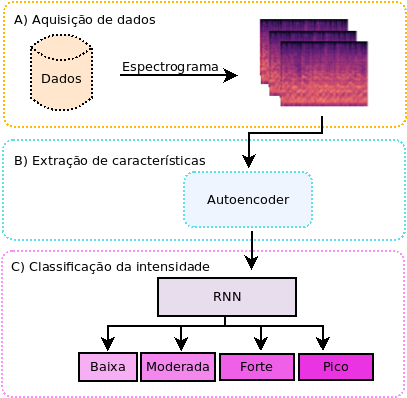
\includegraphics[width=0.75\textwidth]{imagens/arquitetura-visao-geral.png}
\caption{\label{fig:visaogeralproposta}Visão geral da proposta}
\end{figure}

A primeira etapa (A) lida com a obtenção dos dados que serão utilizados no projeto e da sua conversão para uma interpretação passível de utilização por modelos de aprendizagem de máquina. Podemos descrever os dados como um conjunto de registros rotulados que serão utilizados para treinamento, teste e validação dos modelos implementados na proposta.

A segunda etapa (B) lida com a extração de características dos dados convertidos. Essas \textit{features} serão obtidas através de um modelo não supervisionado para a redução de dimensionalidade e posteriormente utilizadas como entrada de um modelo supervisionado de classificação da intensidade da emoção.

A terceira e última etapa (C) é responsável pela inferência da intensidade. O modelo recebe as \textit{features} obtidas na etapa anterior e realiza o treinamento e testagem do modelo de classificação de acordo com quatro classes possíveis: (i) Baixa; (ii) Moderada; (iii) Forte; e (iv) Pico de intensidade.

% ------------------------------------------------------------------------------------------
\subsection{Aquisição dos dados}

O primeiro passo para tarefas de \textit{machine learning} que envolvem \textit{SER} costuma ser a aquisição dos dados que serão utilizados na etapa de criação do modelo. Em virtude do escopo da proposta, necessitamos de um \textit{dataset} em português que possua as classes desejadas: Emoção e intensidade.

Até o momento da escrita deste tabalho, não sabemos de nenhum \textit{dataset} que seja ideal (idioma, emoções e intensidade) para esta proposta. Então, conforme descrito na seção \ref{section:basesdedados}, este trabalho utilizará duas bases de dados: VERBO \cite{12.21} e VIVAE \cite{16}.

O primeiro \textit{dataset}, VERBO, é composto por vocalizações verbais, acomodando todos os fonemas da língua portuguesa, com exemplos para seis emoções básicas (alegria, nojo, medo, raiva, surpresa, tristeza) e um estado emocional denominado de neutro.

O segundo, VIVAE, é composto por vocalizações não verbais distribuidas em seis classes (conquista, prazer sexual, surpresa positiva, raiva, medo e dor física), com exemplos em quatro intensidades (baixa, moderada, fote e pico de intensidade). Graças a fusão de domínios \cite{49}, conseguimos o cenário da Tabela \ref{table:datasetideal}.

Assim, sejam os dois \textit{datasets} VERBO e VIVAE, de modo que VERBO é constituído por pares \{amostra, classe\} e VIVAE por pares \{amostra, classe, intensidade\}, onde as classes são a emoção atribuída àquela amostra, e a intensidade é o rótulo da intensidade da classe daquela amostra. Vamos representar as amostras do VERBO por $X_{VERBO}$ e do VIVAE por $X_{VIVAE}$.

\begin{table}[!h]
\centering
\label{table:datasetideal}
\caption{Atributos dos datasets VERBO, VIVAE, ideal e da fusão de domínios}
\begin{tabular}{l|cccc|}
\cline{2-5}
 & \multicolumn{4}{c|}{Datasets} \\ \hline
\multicolumn{1}{|l|}{Atributos} & \multicolumn{1}{c|}{VERBO} & \multicolumn{1}{c|}{VIVAE} & \multicolumn{1}{c|}{Ideal} & Data Fusion(VERBO,VIVAE) \\ \hline
\multicolumn{1}{|l|}{Idioma} & \multicolumn{1}{c|}{X} & \multicolumn{1}{c|}{} & \multicolumn{1}{c|}{X} & X \\ \hline
\multicolumn{1}{|l|}{Emoções} & \multicolumn{1}{c|}{X} & \multicolumn{1}{c|}{X} & \multicolumn{1}{c|}{X} & X \\ \hline
\multicolumn{1}{|l|}{Intensidade} & \multicolumn{1}{c|}{} & \multicolumn{1}{c|}{X} & \multicolumn{1}{c|}{X} & X \\ \hline
\end{tabular}
\end{table}

Seja $Y_{VERBO}$ o conjunto das classes (emoções) $y_i \forall x_i \in X_{VERBO}$, analogamente para $Y_{VIVAE}$, vamos definir $Y = Y_{VERBO} \bigcap Y_{VIVAE}$. Vamos definir por por $Z$ o conjunto das intensidades. Sabemos das Tabelas \ref{table:vivaeintensidade} e \ref{table:totalporclasse} que

\begin{itemize}
    \item $Y = \{alegria, medo, raiva, supresa\}$
    \item $Z = \{baixa, moderada, forte, pico\}$
\end{itemize}

\begin{figure}[!h]
\centering
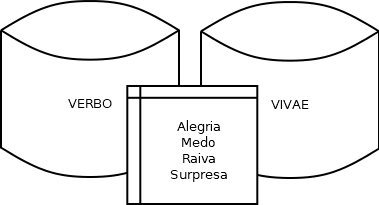
\includegraphics[width=0.40\textwidth]{imagens/p-yverbointeryvivae.png}
\caption{\label{fig:yverbointeryvivae}Interseção entre rótulos de emoções de VERBO e VIVAE}
\end{figure}

Vamos redefinir $X_{VERBO} = \{x_i \mid y_i \in Y\}$, analogamente para $X_{VIVAE}$, e vamos definir nosso domínio $X = X_{VERBO} \bigcap X_{VIVAE}$, assim

\begin{itemize}
    \item $\forall x_i \in X, \exists y_i \in Y$ tal que  $y_i$ é a classe de $x_i$
    \item $\forall x_j \in X_{VIVAE}, \exists z_j \in Z$ tal que  $z_j$ é a intensidade de $x_j$
\end{itemize}

\begin{figure}[!h]
\centering
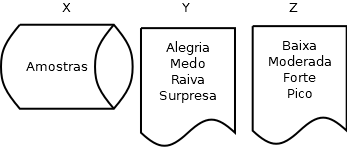
\includegraphics[width=0.5\textwidth]{imagens/p-dominios-contradominos.png}
\caption{\label{fig:dominioscontradominios}Domínio e contradomínios}
\end{figure}

% ------------------------------------------------------------------------------------------
\subsection{Extração de características}

Redes neurais constituem uma boa ferramenta para tarefas de \textit{SER}. CNNs como \textit{feature extractors}, mais ainda \textit{Autoencoders}, que podem criar uma representação de qualidade com dimensionalidade reduzida em seu espaço latente. \textit{DNNs} e \textit{SVM}s encotram espaço na literatura como bons discriminadores e algoritmos não supervisionados como \textit{PCA} e \textit{K-means} podem atuar como formadores de \textit{clusters} para avaliar o desempenho de geração de dados sintéticos.

Os arquivos \textit{.wav} de $X$ serão lidos e iremos gerar seus respectivos \textit{Mel-spectrograms}, formando um mapa $M(x_i): spectrograma_i$.

Vamos construir um \textit{Autoencoder}, $AE$, que tenta reproduzir uma função identendida, e por definição, é composto por uma função \textit{encoder} $f_e$ e uma função $decoder$ $f_d$, de modo que $AE: M \rightarrow M'$ faça

\begin{equation}
    AE(x) = f_d(f_e(x)) = x' \approx x
\end{equation}

\begin{figure}[!h]
\centering
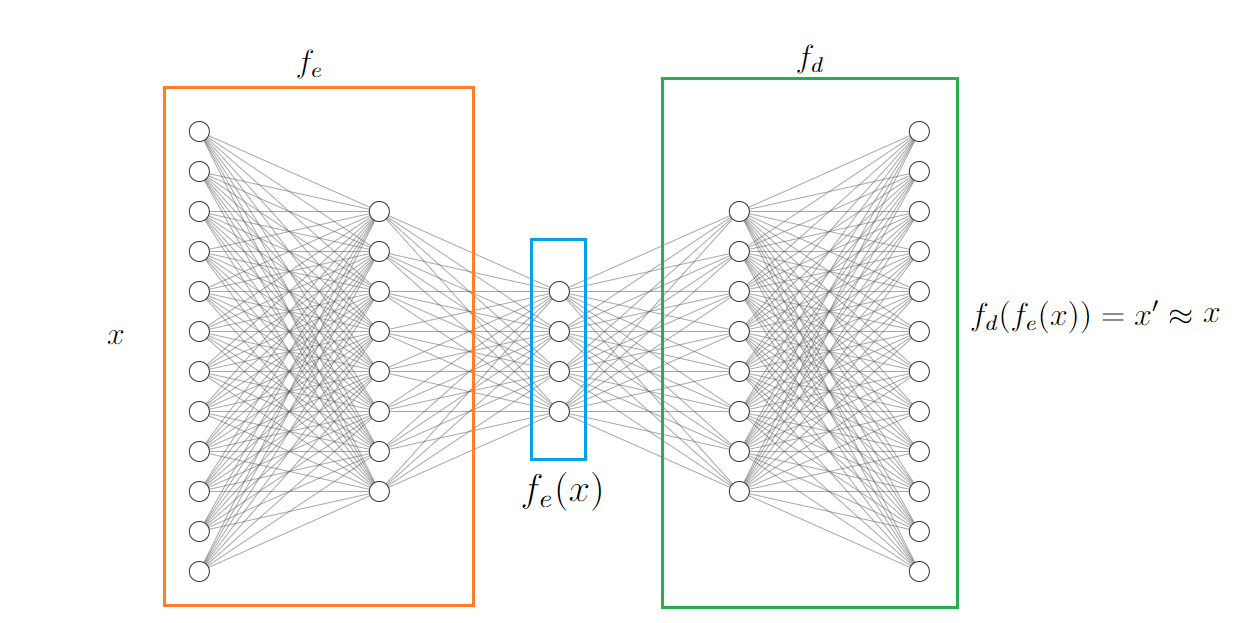
\includegraphics[width=0.9\textwidth]{imagens/p-autoencoder.png}
\caption{\label{fig:treinamentoae}Treinamento do \textit{AE}}
\end{figure}

O modelo $AE$ será treinado no dataset $X$. Após o treinamento, vamos separar $X_{VIVAE}$ em três partes com proporções $0,8$, $0,1$ e $0,1$, que irão formar as amostras de treino ($X_{VIVAE_{treino}}$), teste ($X_{VIVAE_{teste}}$) e validação ($X_{VIVAE_{validacao}}$), respectivamente, do modelo supervisionado $j$ que iremos construir a seguir.

% ------------------------------------------------------------------------------------------
\subsection{Classificação da Intensidade}

Através do modelo de Russel sabemos que que é possível dispor as emoções em função da valência (prazer ou desprazer) e da ativação (vigor ou quietude) \cite{27}. Plutchik decompõe emoções básicas de acordo com a intensidade, chegando a emoções compostas, formadas a partir de duas emoções com intensidades menores.

Conhecemos a miríade de informações que \textit{features} espectrais carregam sobre o som e vimos formas para avaliar o desempenho dos modelos.

Vamos construir e treinar um modelo $j$ supervisionado de classificação (e.g.: \textit{DNN}) que recebe como \textit{input} o \textit{encoding} do \textit{mel-spectrogram} dos $x_i \in X_{VIVAE_{treino}}$ Este modelo será construído para classificar a intensidade da emoção. Uma vez que os $x_i \in X_{VIVAE_{treino}}$ têm correspondentes em $Z$, contra domínio das intensidades, então, $j: M \rightarrow Z$, é tal que

\begin{equation}
    j(f_e(m)) = z
\end{equation}

\begin{figure}[!h]
\centering
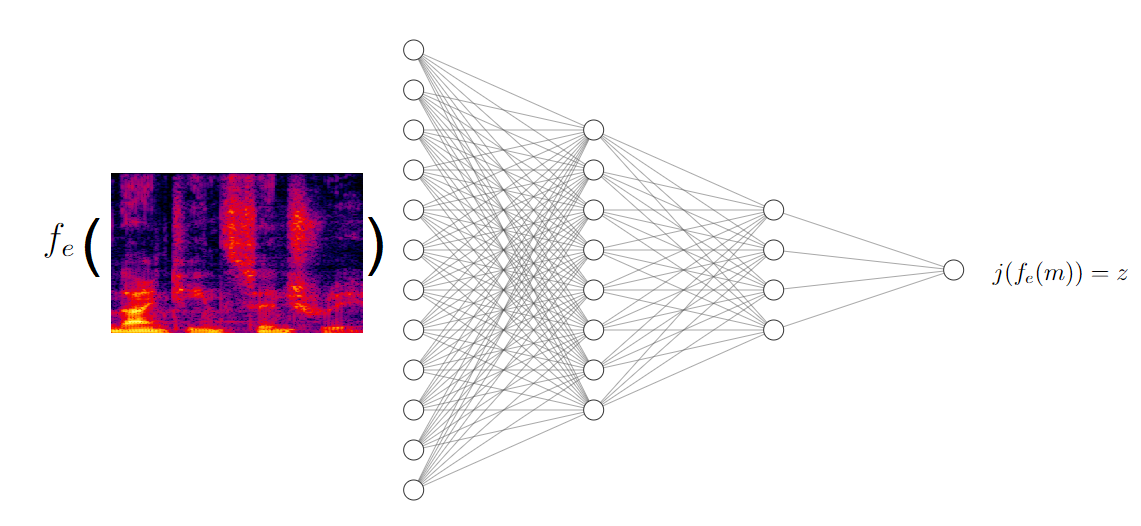
\includegraphics[width=1.0\textwidth]{imagens/p-supervisionado.png}
\caption{\label{fig:jsupervisionado}Modelo supervisionado $j$}
\end{figure}

Por ser tratar de um modelo supervisionado, podemos aplicar as méricas descritas em \ref{sec:metricas}, utilizando $X_{VIVAE_{validacao}}$ e $X_{VIVAE_{teste}}$ para testar e validar seus resultados.

Uma vez que o desempenho de $j$ seja satisfatório, vamos aplicar $j$ em $X_{VERBO}$, obtendo $Z' = \{j(x_i), \forall x_i \in X_{VERBO}\}$. Entretanto, como não existe correspondência entre $X_{VERBO} \rightarrow Z$, não podemos validar imediatamente as intensidades $z'$.

% ------------------------------------------------------------------------------------------
\subsection{Validação}

Como sabemos as intensidades reais $z_i$ dos $x_i \in X_{VIVAE}$, vamos agregar as features e intensidades, formando vetores, $v_i, u_i$, onde

\begin{itemize}
    \item $v_i = [f_e(m_i), z_i]$, onde $x_i \in X_{VIVAE}$
    \item $u_i = [f_e(m_i), j(m_i) = z'_i]$, onde $x_i \in X_{VERBO}$
\end{itemize}

Portanto, devemos ter vetores $u,v$ que contêm em atributos representativos de características relativas a emoção e a intensidade dessa emoção.

Podemos então aplicar técnicas de clusterização (e.g.: \textit{PCA}) para investigar se os vetores com classe ($y$) e intensidade ($z$) são agrupáveis de forma coerente com base em suas características $y, z$ e verificar a validade de $j$ em $X_{VERBO}$.

\begin{figure}[!h]
\centering
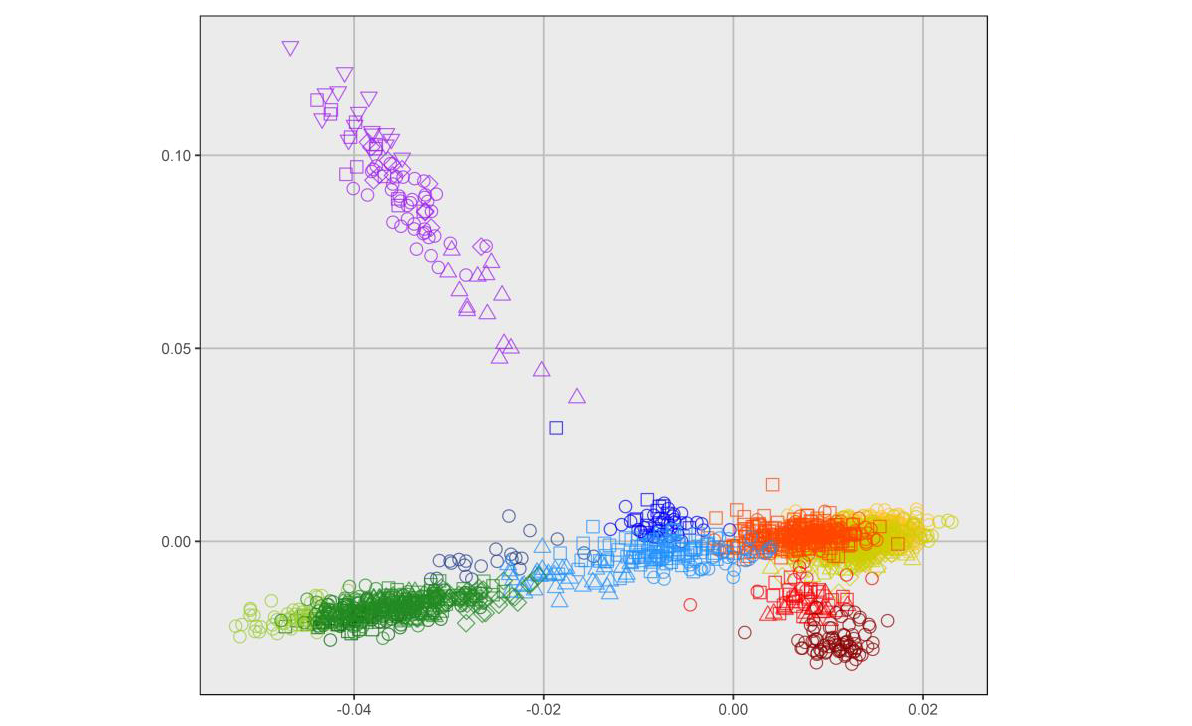
\includegraphics[width=1.0\textwidth]{imagens/p-naosupervisionado.png}
\caption{\label{fig:clusterizacaoresults}Exemplo de clusterização de resultados}
\end{figure}

\clearpage
% ==========================================================================================
\section{Plano de Trabalho e Cronograma}

Esta seção apresenta as atividades propostas para este projeto de pesquisa, juntamente com um cronograma de acompanhamento. Planeja-se finalizar o projeto em dois anos de atividades. Abaixo, temos enumeradas as atividades necessárias para a conclusão do Programa de Pós-Graduação em Informática da Universidade de Brasília (PPGI/UnB) e obtenção do título de Mestre. A Tabela \ref{table:cronogramaproposta} apresenta o cronograma de atividades deste plano de trabalho.\\

Atividades:

\begin{enumerate}
    \item Obtenção dos créditos obrigatórios exigidos pelo programa de mestrado;
    \item Obtenção da certificação de proficiência em idioma Inglês;
    \item Revisão da literatura, fundamentação teórica e apresentações;
    \item Redação e exame da qualificação;
    \item Planejar, realizar e analisar os experimentos;
    \item Publicação dos resultados;
    \item Redação da dissertação e defesa do mestrado.
\end{enumerate}

\begin{table}[!h]
\centering
\label{table:cronogramaproposta}
\caption{Cronograma proposto de atividades, onde \textbf{X} representa atividades finalizadas e \textbf{O} representa atividades a desenvolver}
\label{tab:my-table}
\begin{tabular}{ccccccccc}
\cline{3-9}
 & \multicolumn{1}{c|}{} & \multicolumn{7}{c|}{Atividade no trimestre} \\ \hline
\multicolumn{2}{|c|}{Período} & \multicolumn{1}{c|}{1} & \multicolumn{1}{c|}{2} & \multicolumn{1}{c|}{3} & \multicolumn{1}{c|}{4} & \multicolumn{1}{c|}{5} & \multicolumn{1}{c|}{6} & \multicolumn{1}{c|}{7} \\ \hline
\multicolumn{1}{|c|}{\multirow{2}{*}{2022}} & \multicolumn{1}{c|}{3o trimestre} & \multicolumn{1}{c|}{X} & \multicolumn{1}{c|}{} & \multicolumn{1}{c|}{} & \multicolumn{1}{c|}{} & \multicolumn{1}{c|}{} & \multicolumn{1}{c|}{} & \multicolumn{1}{c|}{} \\ \cline{2-9} 
\multicolumn{1}{|c|}{} & \multicolumn{1}{c|}{4o trimestre} & \multicolumn{1}{c|}{X} & \multicolumn{1}{c|}{X} & \multicolumn{1}{c|}{X} & \multicolumn{1}{c|}{X} & \multicolumn{1}{c|}{X} & \multicolumn{1}{c|}{} & \multicolumn{1}{c|}{} \\ \hline
\multicolumn{1}{|c|}{\multirow{4}{*}{2023}} & \multicolumn{1}{c|}{1o trimestre} & \multicolumn{1}{c|}{X} & \multicolumn{1}{c|}{} & \multicolumn{1}{c|}{O} & \multicolumn{1}{c|}{} & \multicolumn{1}{c|}{O} & \multicolumn{1}{c|}{} & \multicolumn{1}{c|}{} \\ \cline{2-9} 
\multicolumn{1}{|c|}{} & \multicolumn{1}{c|}{2o trimestre} & \multicolumn{1}{c|}{X} & \multicolumn{1}{c|}{} & \multicolumn{1}{c|}{O} & \multicolumn{1}{c|}{} & \multicolumn{1}{c|}{O} & \multicolumn{1}{c|}{} & \multicolumn{1}{c|}{} \\ \cline{2-9} 
\multicolumn{1}{|c|}{} & \multicolumn{1}{c|}{3o trimestre} & \multicolumn{1}{c|}{X} & \multicolumn{1}{c|}{} & \multicolumn{1}{c|}{O} & \multicolumn{1}{c|}{} & \multicolumn{1}{c|}{O} & \multicolumn{1}{c|}{O} & \multicolumn{1}{c|}{} \\ \cline{2-9} 
\multicolumn{1}{|c|}{} & \multicolumn{1}{c|}{4o trimestre} & \multicolumn{1}{c|}{X} & \multicolumn{1}{c|}{} & \multicolumn{1}{c|}{O} & \multicolumn{1}{c|}{} & \multicolumn{1}{c|}{O} & \multicolumn{1}{c|}{O} & \multicolumn{1}{c|}{} \\ \hline
\multicolumn{1}{|c|}{\multirow{2}{*}{2024}} & \multicolumn{1}{c|}{1o trimestre} & \multicolumn{1}{c|}{X} & \multicolumn{1}{c|}{} & \multicolumn{1}{c|}{} & \multicolumn{1}{c|}{} & \multicolumn{1}{c|}{} & \multicolumn{1}{c|}{O} & \multicolumn{1}{c|}{O} \\ \cline{2-9} 
\multicolumn{1}{|c|}{} & \multicolumn{1}{c|}{2o trimestre} & \multicolumn{1}{c|}{X} & \multicolumn{1}{c|}{} & \multicolumn{1}{c|}{} & \multicolumn{1}{c|}{} & \multicolumn{1}{c|}{} & \multicolumn{1}{c|}{O} & \multicolumn{1}{c|}{O} \\ \hline
\multicolumn{1}{l}{} & \multicolumn{1}{l}{} & \multicolumn{1}{l}{} & \multicolumn{1}{l}{} & \multicolumn{1}{l}{} & \multicolumn{1}{l}{} & \multicolumn{1}{l}{} & \multicolumn{1}{l}{} & \multicolumn{1}{l}{} \\
\multicolumn{1}{l}{} & \multicolumn{1}{l}{} & \multicolumn{1}{l}{} & \multicolumn{1}{l}{} & \multicolumn{1}{l}{} & \multicolumn{1}{l}{} & \multicolumn{1}{l}{} & \multicolumn{1}{l}{} & \multicolumn{1}{l}{}
\end{tabular}
\end{table}

\chapter{Fundamentação Teórica}\label{Cap:Fundamentação Teórica}

Neste capítulo serão expostos conceitos necessários para a compreensão deste trabalho. Iniciando pelo processo de formação da voz e conceituando formas como as emoções são catalogadas. Em seguida, uma exposição de conceitos relativos a Aprendizado de Máquina e Aprendizado Profundo, algumas de suas arquiteturas e abordagens para iniciar as tarefas com esse tipo de tecnologia. Vamos discorrer sobre os dados, material essencial para trabalhos envolvendo aprendizado de máquina. Veremos formas forma de processar esses dados e, por fim, técnicas para aferir a eficiência de tarefas de Aprendizado de Máquina.\\

% ==========================================================================================
\section{Voz, Emoção e Intensidade}

A voz humana é produzida na laringe. Com a passagem do ar - oriundo dos pulmões - pelas pregas ("cordas") vocais, estas vibram e geram um som. Com o auxílio de outras estruturas fisiológicas como língua, boca e lábios, esse som é transformado e nossa voz é produzida \cite{51}. A fala não é somente um ato de expressão de ideias e emoções por meio da vocalização \cite{6.31}, como também é um componente indispensável para a comunicação entre os indivíduos de uma sociedade. Enquanto humanos, somos especialistas em voz, e conseguimos extrair uma gama de informações socialmente relevantes \cite{49} dessas ondas sonoras.

Nas emoções, temos três modelos bastante consolidados na literatura: Ekman, Russel, e Plutchik.

O modelo de Ekman \cite{31.9} afirma existirem seis emoções básicas: Neutra, raiva, medo, surpresa, alegria e tristeza. E que estas são reconhecidas independentemente do idioma, da cultura ou dos meio de expressão (i.e.: fala, expressões faciais, etc.). Há o modelo de Russel \cite{31.10} (Figura \ref{fig:russel}), que sugere que as emoções podem ser representadas em um espaço bidimensional, onde o eixo horizontal representa a valência (positiva ou negativa) e o eixo vertical representa a ativação (alta ou baixa). Também podemos citar o modelo de Plutchik \cite{57} (Figura \ref{fig:plutchik}), que combina os dois modelos anteiores, criando emoções internas (básicas ou primárias) e externas (compostas ou secundárias).

No modelo de Russel, que dispõe as emoções ao longo desses dois eixos (valência e ativação), as
emoções que se encontram mais próximas apresentam uma maior correlação de um desses atributos e no o seu centro fica representado um estado de neutralidade.

Plutchik extendeu \cite{57} o modelo de Russel. Seu modelo, em formato de cone, dispõe de oito emoções básicas com cores distintas. Neste modelo, a intensidade da emoção fica denotada pela intensidade da cor naquela região, indo do mais intenso (centro) para o menos intenso (borda), por exemplo: Com relação ao medo, o terror é mais intenso que a apreensão. As emoções estão dispostas de acordo com seu grau de similaridade: As mais similares estão próximas e as mais antagônicas estão diametralmente opostas. No modelo de Plutchick, as emoções compostas, são aquelas formadas por duas emoções básicas.

A intensidade da emoção pode afetar nossa percepcão da mesma \cite{18.46}. Por exemplo: Felicidade pode ser confundida com euforia, que são semelhantes em qualidade de voz mas distintas quanto a intensidade \cite{18.9}. Correlacionar a intensidade da emoção com o volume da voz é demasiada simplificação. A intensidade da emoção não pode ser inferida apenas pela energia na fala \cite{18.12}. As diferenças entre características acústicas da voz podem ser maiores entre diferentes intensidades de uma mesma emoção do que entre emoções diferentes \cite{18.46}.

Do ponto de vista do comportamento social, \cite{16} diz que uma representação da ativação e da intensidade do estado emocional parecem essenciais, mesmo quando a valência não pode ser determinada.

\begin{figure}[!ht]
\centering
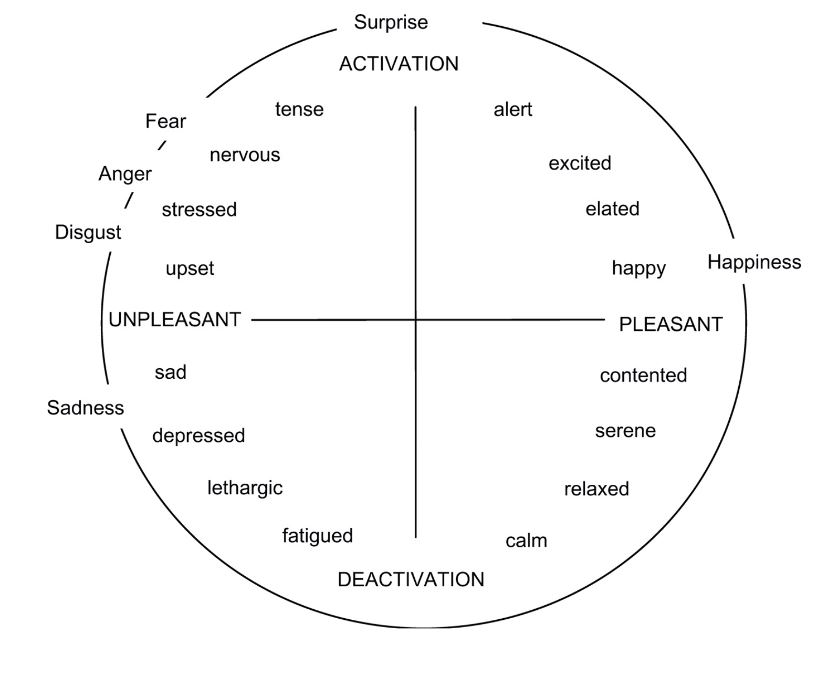
\includegraphics[width=0.6\textwidth]{imagens/russel.JPG}
\caption{\label{fig:russel}Modelo de Russel \cite{25}}
\end{figure}

\begin{figure}[!h]
\centering
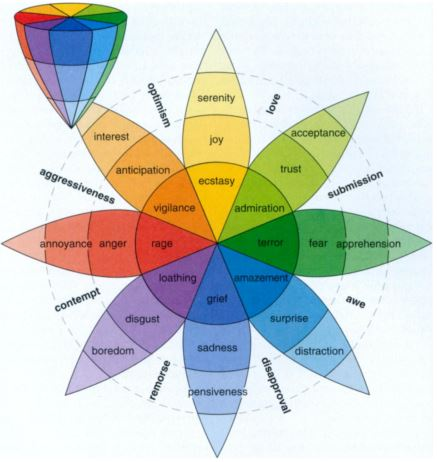
\includegraphics[width=0.7\textwidth]{imagens/plutchik.JPG}
\caption{\label{fig:plutchik}Modelo de Plutchik \cite{57}}
\end{figure}

% ==========================================================================================
\section{Aprendizado de Máquina}

O Aprendizado de Máquina (\textit{Machine Learning}, \textit{ML}) é uma subárea da Inteligência Artificial (\textit{Artificial Intelligence}, \textit{AI}). Inteligência Artificial foi o nome estabelecido \cite{12.23} para uma área denominada Inteligência Computacional, que consiste no estudo agentes inteligentes. Um agente é algo capaz de atuar num ambiente, enquanto um agente inteligente é um agente que atua no ambiente de forma inteligente, se apropriando de circunstâncias para alcançar um objetivo, possivelmente influenciando o ambiente, com capacidade para alterar esse objetivo, aprendendo com sua experiência e fazendo escolhas adequadas de acordo com suas limitações.

Tarefas de \textit{ML} costumam ser descritas em termos de como o sistema de aprendizado de máquina deve processar um exemplo \cite{53}. Um exemplo consiste numa coleção de recursos, de um objeto ou evento, que foram aferidos quantitativamente e que desejamos que seja processado por esse sistema. Costuma-se representar um exemplo como um vetor $x \in R^n$, onde cada coordenada $x_i$ do vetor $x$ é uma característica (\textit{feature}) desse vetor. Por exemplo, se $x$ representar uma imagem, cada $x_i$ pode ser o valor de um pixel dessa imagem.

Dentre as tarefas de \textit{ML}, duas tarefas comuns são a classificação e a regressão. A classificação busca descobrir a qual de $k$ classes possíveis um vetor $x$ pertence, produzindo uma função $f: R^n \rightarrow \{1, ..., k\}$, de modo que quando $y = f(x)$, o modelo atribui a uma entrada (\textit{input}) $x$ uma saída (\textit{output}) numérica de valor $y$ que representa uma categoria (classe). Na regressão, o pensamento é análogo, porém, ao final, o modelo não tenta encontrar a qual classe $x$ pertence, e sim predizer um valor (contínuo) para $f(x)$.

Diversos algoritmos de \textit{ML} foram investigados em trabalhos de SER \cite{20.7}, como Floresta Aleatória (\textit{Random Forest}, \textit{RF}) em \cite{20.10}, Árvore de Decisão \cite{20.11} (\textit{Decision Tree}), Máquinas de Vetor de Suporte \cite{20.13} (\textit{Support Vector Machines}, \textit{SVM}), K-vizinhos mais próximos \cite{20.15} (\textit{K-Nearest Neighbors}, \textit{KNN}) e Classificador de Aumento de Gradiente [20.16 (\textit{Gradient Boosting Classifier}, \textit{GBC}).

% ==========================================================================================
\section{Deep Learning e Redes Neurais}

Aprendizado Profundo (\textit{Deep learning}, \textit{DL}) é um tipo específico de ML \cite{53}. Algoritmos de ML citados no parágrafo anterior - conhecidos como algoritmos tradicionais - costumam funcionar bem em uma grande variedade de problemas importantes. Entretanto, não costumam ter desepenho tão bom em problemas que envolvem reconhecimento de fala ou de objetos. O desenvolvimento do \textit{DL} foi motivado, em parte, pela falha desses algoritmos tradicionais em generalizar bem para essas tarefas de IA.

Dada essa necessidade de explorar modelos mais robustos, alguns trabalhos estudaram o impacto de algoritmos de \textit{DL} no reconhecimento de emoção na voz \cite{12.12} \cite{12.16}.

\begin{figure}[!h]
\centering
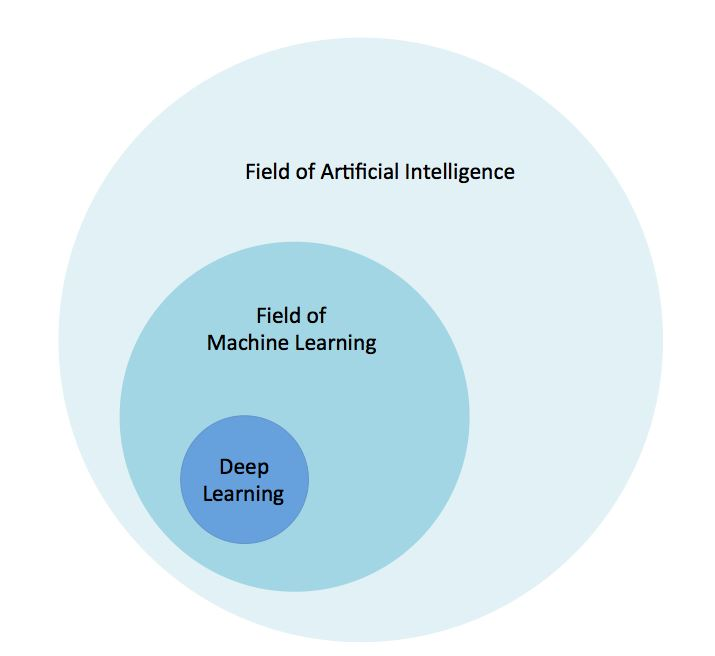
\includegraphics[width=0.5\textwidth]{imagens/ia-ml-dl.JPG}
\caption{\label{fig:ia-ml-dl}Relação entre \textit{IA}, \textit{ML} e \textit{DL}}

\author{Fonte: Retirada de \cite{58}}
\end{figure}

Redes Multicamadas de Perceptrons (\textit{Multilayer Perceptron}, \textit{MLP}) são a pedra fundamental na construção de modelos de \textit{DL}, conhecidos como Redes Neurais (\textit{Neural Networks}, \textit{NN}). O Perceptron é uma unidade (Figura \ref{fig:perceptron}) composta por valores (pesos) $wi$ e uma função de ativação $f$,  que recebe as \textit{fetures}, realiza uma operação matemática entre $wi,xi$, aplica a função de ativação $y = f(x,w)$ e emite esse resultado como \textit{output}.

Podemos realizar o mapeamento de vários Perceptrons, recebendo as \textit{features} e preoduzindo \textit{outputs}, ao longo de camadas, onde cada camada atua como \textit{input} para a próxima camada, e assim sucessivamente, até chegar a um \textit{output} final, assim, temos uma \textit{MLP} (Figura\footnote{Imagem adaptada, gerada em \url{http://alexlenail.me/NN-SVG/index.html}}\ref{fig:mlp}). A camada inicial é chamada de camada de entrada (\textit{input layer}), as camadas intermediárias são chamadas de camdas ocultas (\textit{hidden layers}) e à camada final chamamos camada de saída (\textit{output layer}). Compreendendo uma rede neural como um conjunto de nós e arestas, cada nó da rede será chamado de neurônio.

\begin{figure}[!ht]
\centering
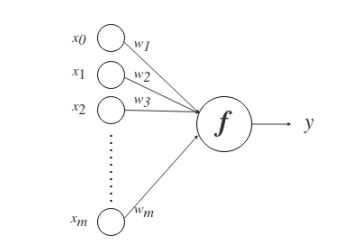
\includegraphics[width=0.6\textwidth]{imagens/perceptron.png}
\caption{\label{fig:perceptron}Exemplo de Perceptron}

\author{Fonte: Retirado de \cite{12}}
\end{figure}

\begin{figure}[!h]
\centering
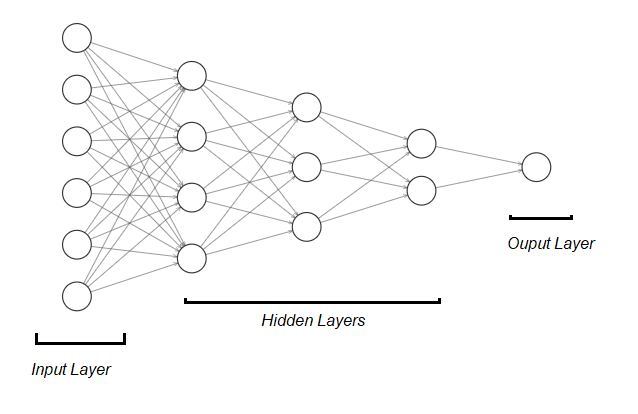
\includegraphics[width=0.75\textwidth]{imagens/mlp02.png}
\caption{\label{fig:mlp}Exemplo de arquitetura \textit{MLP}}

\end{figure}

% ------------------------------------------------------------------------------------------
\subsection{Redes Neurais Profundas}

Nosso cérebro tem uma grande capacidade de generaliação, o que nos ajuda a raciocinar de forma indutiva e é o primeiro passo do nosso aprendizado \cite{32}. Redes neurais são capazes de aprender relações não-lienares complexas e criar relações entre \textit{input} e \textit{output}, formando sistemas utilizados em várias áreas de \textit{ML}, e \textit{SER} não é uma exceção \cite{32.74}.

Com base no conceito e organização de uma rede neural, o conjunto formado pela disposição dos neurônios, pesos e funções de ativação pode ser organizado de forma a criar diferentes arquiteturas\footnote{Exemplos visuais de diversas arquiteturas de DL: \url{https://www.asimovinstitute.org/neural-network-zoo/}}, que ao longo do tempo se mostraram eficientes para generalizar bem em certas áreas de conhecimento. Diremos que uma rede neural se torna uma Rede Neural Profunda (\textit{Deep Neural Network}, \textit{DNN}) (Figura\footnote{Gerada em \url{http://alexlenail.me/NN-SVG/index.html}} \ref{fig:exarqdnn}) quando possue grande quantidade de neurônios e camadas ocultas em sua arquitetura, embora não haja um valor específico que a habilite a se tornar profunda ao superá-lo.

\begin{figure}[!h]
\centering
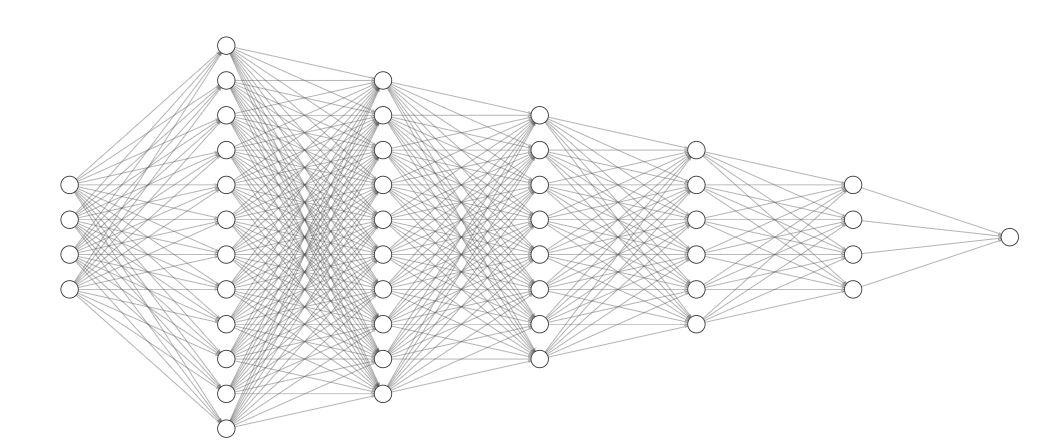
\includegraphics[width=1.0\textwidth]{imagens/ex-dnn.JPG}
\caption{\label{fig:exarqdnn}Exemplo de arquitetura \textit{DNN}}
\end{figure}

A seguir, abordaremos duas dessas arquiteturas que se mostram importantes para este trabalho: Redes Neurais Convolucionais e Autoencoder.

% ------------------------------------------------------------------------------------------
\subsection{Redes Neurais Convolucionais}

Redes Neurais Convolucionais\footnote{Introduzido em 1989 por Y. LeCun \textit{et al.}} (\textit{Convolutional Neural Networks}, \textit{CNN}), também conhecidas como Redes Convolucionais, são um tipo de rede neural especializada para processar dados que tenha uma topologia semelhante a um formato de grade. Dados como esses podem ser, por exemplo, imagens ou séries temporais. Poderíamos interpretar uma leitura numa série temporal num instante $t$ como uma coluna, e, assim, acumular horizontalmente essas leituras ao longo do tempo criando uma estrutura que atenda a esse padrão de gradem. Enquanto numa imagem, podemos interpretar os valores dos pixels como elementos que formam essa mesma estrutura. Um exemplo de uma arquitetura de \textit{CNN} pode ser observado na Figura\footnote{Gerada em \url{http://alexlenail.me/NN-SVG/LeNet.html}} \ref{fig:exarqcnn}.

O nome convolucional vem da operação de Convolução, uma operação linear entre duas funções $f$ e $g$ que produzem uma terceira função $f*g$ e que expressa como o formato de $f$ é influenciado por $g$. A operação de convolução é definida como:

\begin{equation}
(f*g)(t) \coloneqq \int^{-\infty}_{\infty}{f(a) * g(t - a) \partial{da}}
\end{equation}

Costumeiramente, nos referimos a convolução apenas através de $(f*g)(t)$, onde $f$ é nosso \textit{input}, $g$ será o nosso filtro (\textit{kernel}),  e o resultado (\textit{output}) da convolução costuma ser chamado de mapa de características (\textit{feature map}). Um exemplo de convolução pode ser observado na Figura \footnote{Imagem retirada de \url{https://courses.cs.washington.edu/courses/cse446/22wi/sections/08/convolutional_networks.html}} \ref{fig:2dconv}. Perceba que \textit{output} foi obtido movendo (deslizando) o \textit{kernel} ao longo das linhas e colunas do \textit{input}, realizando, a cada iteração, a soma do produto dos elementos sobrepostos entre o \textit{input} e o \textit{kernel}.

\begin{figure}[!h]
\centering
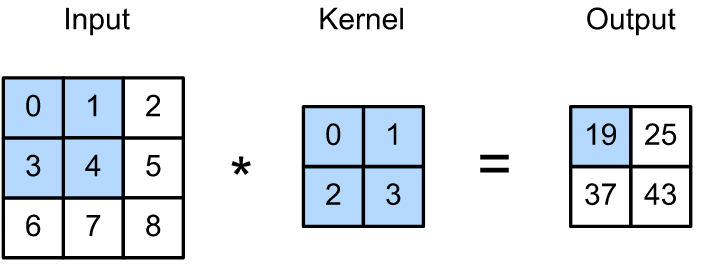
\includegraphics[width=0.7\textwidth]{imagens/2dconv.png}
\caption{\label{fig:2dconv}Exemplo de Convolução}
\end{figure}

\begin{figure}[!h]
\centering
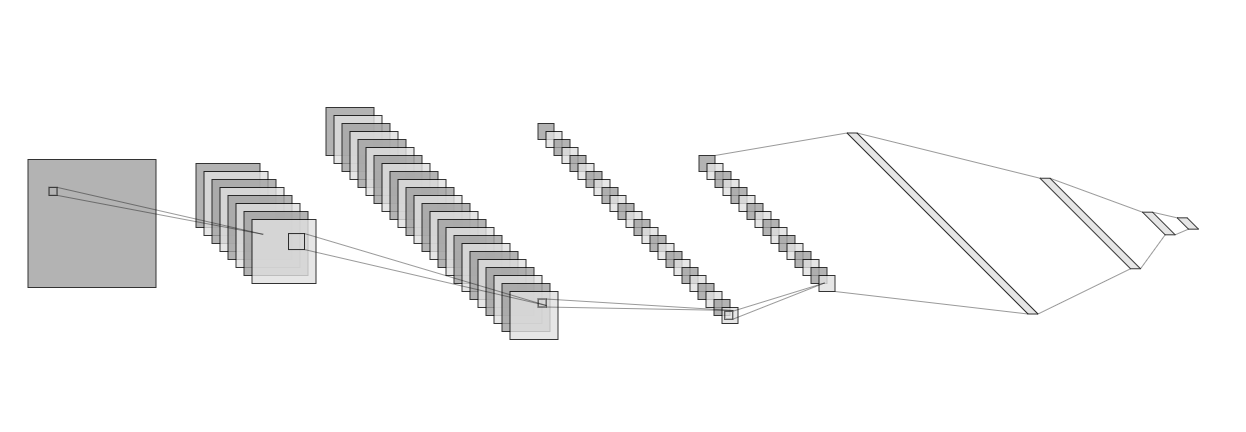
\includegraphics[width=1.0\textwidth]{imagens/ex-cnn.png} % https://towardsdatascience.com/applied-deep-learning-part-3-autoencoders-1c083af4d798
\caption{\label{fig:exarqcnn}Exemplo de arquitetura \textit{CNN}}
\end{figure}

Redes Neurais Convolucionais são populares em trabalhos envolvendo SER \cite{37.125} \cite{37.126} \cite{37.127} \cite{37.128}, e sua capacidade de generalização de características se mostra superior a abordagens puras de \textit{DNN} \cite{37.50}.

% ------------------------------------------------------------------------------------------
\subsection{Codificador Automático}

Um Codificador Automático (\textit{Autoencoder}, \textit{AE}) é uma rede neural criada para tentar reproduzir o seu \textit{input} no seu \textit{output}. Podemos descrever um \textit{AE} como um conjunto de funções $f, f'$ de modo que, dado um input $x$, queremos $f'(f(x)) = x' \approx x$, onde $f$ realiza a codificação (\textit{encoding}) de $x$ e $f'$ realiza a decodificação (\textit{decoding}) do resultado $f(x)$. Assim, um \textit{AE} é uma rede neural composta por um \textit{encoder} e um \textit{decoder} (Figura\footnote{Imagem adaptada, gerada em \url{http://alexlenail.me/NN-SVG/LeNet.html}} \ref{fig:exarqae}) que tenta reproduzir uma função de identidade.

O resultado da etapa de \textit{encoding} costuma ter uma dimensionalidade menor do que a do dado de entrada. O espaço composto por dados codificados (\textit{encoded}) é chamado de Espaço Latente (\textit{Latent Space}), um espaço composto por representações significativas dos dados, contendo informações sobre cada amostra que possivelmente não estariam visíveis nas representações de alta dimensionalidade \cite{60}.

Entretanto, \textit{Autoencoder}s não podem simplesmente aprender a generalizar $f'(f(x)) = x$ para todo tipo de dado, ao invés disso, são impostas restrições para que consigam esse tipo de generalização apenas para os dados relevantes a sua tarefa. Forçando o modelo a priorizar características que devem ser aprendidas, por vezes, ele aprende propriedades úteis sobre os dados.

Tradicionalmente, \textit{Autoencoder}s foram utilizados para reduzir a dimensionalidade de dados (\textit{dimensionality reduction}) ou para aprender características (\textit{feature learning}) sobre os dados. Atualmente, \textit{AE} são bastante utilizados como peça fundamental em Redes Generativas Adversariais \footnote{Introduzido em 2014 por Ian J. Goodfellow \textit{et al.}. Disponível em \url{https://arxiv.org/abs/1406.2661}} (\textit{Generative Adversarial Network}, \textit{GAN}) e \textit{Autoencoder}s Variacionais\footnote{Introduzido em 2013 por Diederik P Kingma e Max Welling. Disponível em \url{https://arxiv.org/abs/1312.6114}} (\textit{Variational Autoencoder}, \textit{VAE}).

\begin{figure}[!h]
\centering
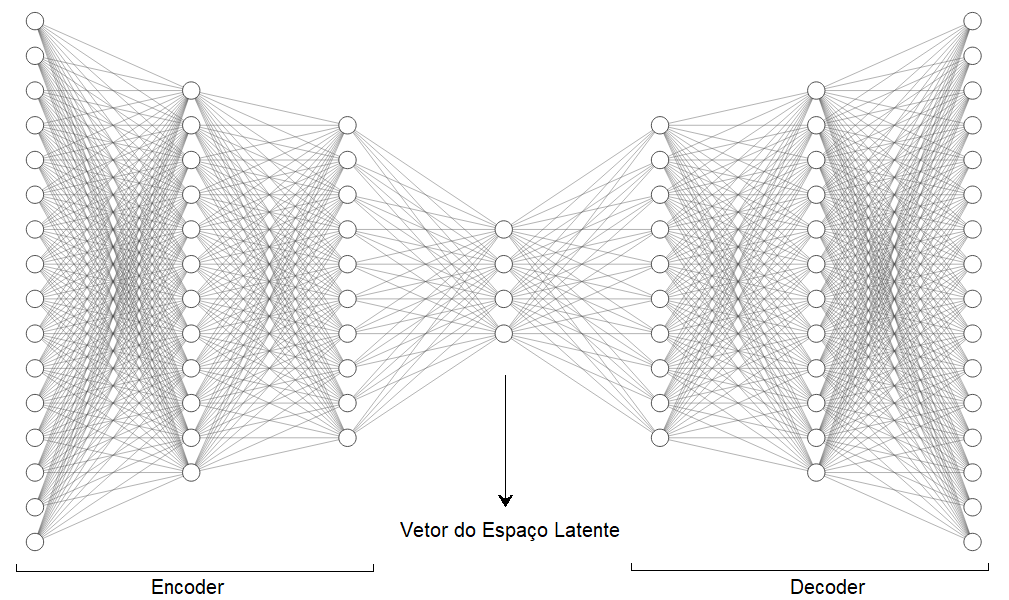
\includegraphics[width=1.0\textwidth]{imagens/ex-ae.PNG}
% \caption{\label{fig:exarqae}Exemplo de arquitetura \textit{AE}, com \textit{encoder}, \textit{decoder} e vetor do espaço latente}
\caption{\label{fig:exarqae}Exemplo de arquitetura \textit{AE}}
\end{figure}

% ==========================================================================================
\section{Abordagem: Supervisionada vs. Não Supervisionada}

No processo de criação de modelos de \textit{ML}, uma vez definida a arquitetura, a rede irá começar a aprender com os dados de forma iterativa. A etapa onde o modelo começa a ver os \textit{inputs} e tentar inferir a classe é chamada de treinamento (\textit{training}). Duas abordagens tradicionais para esse momento são a Aprendizagem Supervisionada (Supervised Learning) e a Aprendizagem Não Supervisionada (Unsupervised Learning).

% ------------------------------------------------------------------------------------------
\subsection{Abordagem Supervisionada}\label{supervisionada}

Para a primeira, é necessário que os dados já estejam rotulados com a classe (\textit{label}) a qual cada registro de pertence. Por exemplo, ao utilizar uma base de dados que envolve imagens, pode ser trivial etiquetar os dados com base no objeto que aparece naquela imagem (e.g.: ou gato ou cachorro). Para emoções essa atividade irá demandar pessoas especializadas e capacitadas. Uma pesquisa \cite{32} recente (2021) aponta essa dificuldade na área de \textit{SER}, pois mesmo quando há variedade de conjuntso de dados (\textit{datasets}) diferentes, estes podem apresentar poucas classes, poucos registros por classe ou ambos.

Sejam $X, Y$, conjuntos de \textit{inputs} e \textit{outputs}, respectivamente, $X=\{x_i, ..., x_n\}$ e $Y=\{y_i, ..., y_n\}$, onde o $y_i$ é a classe de $x_i$, podemos generalizar a etapa de treinamento como seguinte fluxo $\forall x_i \in X' \subset X$:

Seja $f: X \rightarrow Y,$ tal que $f(x) = y$, então,

\begin{enumerate}
    \item O modelo $f$ é apresentado a um dado $x_i$ e produz um resultado $f(x_i) = y_i'$;
    \item É calculado um erro $d_i = d(y_i, y_i')$ entre o resultado apresentado e o resultado esperado;
    \item $d_i$ É utilizado para atualizar os parâmetros de $f$;
    \item O processo é repetido para o próximo exemplo $x_{i+1}$.
\end{enumerate}

A etapa de treinamento costuma ser serguida pela etapa de testes (\textit{tests}), onde o modelo é exposto aos $x_j \in (X \setminus X')$ e, a partir daí, são calculadas métricas para aferir o desempenho de $f$.

Cabe observar que $f$ não precisa ser injetora, uma vez que mais de um $x_i$ pode pertencer a mesma classe $y_i$.

\subsection{Abordagem Não Supervisionada}

Para uma abordagem não supervisionada, os modelos são apresentados a um conjunto de dados sem rótulos e tentam aprender características importantes da sua estrutura. A distinção entre supervisionado e não supervisionado costuma se dar pela presença ou não da classe (\textit{target}) daqueles dados. Note que é possível aplicar uma abordagem não supervisionada a um \textit{dataset} mesmo quando a classe é conhecida, basta excluí-la do processo de treinamento do modelo.

Alguns casos de uso de \textit{Unsupervised Learning} incluem: (1) Formação de conjuntos (\textit{clustering}); (2) \textit{Feature Learning}; (3) Redução de dimensionalidade; (4) Automatizar a rotulação de amostras; (5) Aprender sobre o \textit{dataset} através de análise exploratória (\textit{Exploratory Data Analysis}, \textit{EDA}).

Trabalhos envolvendo aprendizado não supervisionado apontam as capacidades do \textit{AE} tanto para \textit{feature learning} \cite{35.16} \cite{35.17} quanto para redução de dimensionalidade \cite{35.18} \cite{35.19}.

% ==========================================================================================
\section{Base de Dados}\label{section:basesdedados}

Para modelar a intensidade da emoção, uma das dificuldades é a falta de dados rotulados \cite{18}. Tradicionalmente, em áreas como visão computadional ou reconhecimento de voz, os \textit{datasets} chegam a ter milhões de registros, como, por exemplo: ImageNet\footnote{Disponível em \url{https://www.image-net.org/about.php}} (imagem) com  mais de 14 milhões e Google AudioSet\footnote{Disponível em \url{http://research.google.com/audioset/}} (áudio) com mais de 2 milhões de amostras. Podemos ver um comparativo na Tabela \ref{table:comparativodbs} entre datasets populares \cite{32} em trabalhos de \textit{SER}: AudioSet, Berlin Database of Emotional Speech (EMO-DB) \cite{32.55}, Danish emotional speech database (DES) \cite{32.56}, The Ryerson Audio-Visual Database of Emotional Speech and Song (RAVDESS) \cite{32.57}, Toronto Emotional Speech Set (TESS) \cite{32.58} e Crowd-Sourced Emotional Multimodal Actors Dataset (CREMA-D) \cite{32.59}.

\begin{table}[!ht]\label{table:comparativodbs}
\centering
\caption{Comparativos entre \textit{datasets} populares para \textit{SER}}
    \begin{tabular}{|l|c|c|c|}
    \hline
        Nome & Quantidade de amostras & Duração Média (s) & Português?  \\ \hline
        EMO-DB  & 700 & 2,8 & Não  \\ \hline
        DES  & 210 & 2,7 & Não  \\ \hline
        RAVDESS  & 2496 & 3,7 & Não  \\ \hline
        TESS  & 2800 & 2,1 & Não  \\ \hline
        CREMA-D  & 7442 & 2,5 & Não  \\ \hline
    \end{tabular}
\end{table}

Não obstante nenhum destes ser em português, língua falada pela sexta\footnote{Disponível em \url{https://brasilescola.uol.com.br/geografia/populacao-mundial.htm}} maior população e nona\footnote{Disponível em \url{https://www.gov.br/funag/pt-br/ipri/publicacoes/estatisticas/as-15-maiores-economias-do-mundo}} maior economia do mundo, podemos observar com facilidade o quão distante estão do AudioSet, tanto em quantidade de amostras ($> 2.000.000$) quanto em duração média ($\approx 10s$).

Todos esses \textit{datasets} são simulados (\textit{simulated}), ou seja, os áudios são gravados a partir de pessoas treinadas lendo um texto e interpretando com emoções diferentes. Existem também datasets seminaturais (\textit{semi-natural}), composto tanto por atores como pessoas comuns lendo um roteiro; e os dito naturais (\textit{natural}), com áudios extraídos de programas de TV, centrais telefônicas, vídeos da internet e outros meios.

Também é comum que as amostras não apresentem ruídos ou alguma puluição sonora, o que as distancia de situações reais. Sistemais treinados neses datasets podem não ser bem sucedidos em situações reais \cite{32}. Há também \textit{datasets} gerados a partir da particiação de um usuário ou cliente de algum serviço, entretanto, este é informado da gravação, o que pode comprometer a qualidade do dado.

Outro problema é o efeito da cultura e da linguagem, onde ambos os fatores podem afetar a percepcão do sentimento na fala \cite{32}. A incerteza na anotação (categorização dos dados) representa mais um desafio para \textit{datasets} de \textit{SER}, uma vez que num discurso emocional, um participante pode rotular um enunciado com \textit{eufórico} e outro como \textit{raivoso}. Essa subjetividade torna a tarefa mais complexa e pode limitar a possibilidade de misturar os bancos de dados para criar superconjuntos de dados emocionais.

% ------------------------------------------------------------------------------------------
\subsection{Fusão de Domínios}

Dado esse cenário, podemos tentar utilizar uma ténica que permite fundir o conhecimento de vários conjuntos de dados organicamente para uma tarefa de aprendizado de máquina. Fusão de Domínios \cite{49}(\textit{Domain Fusion}) é uma técnica para aproveitar mais bases de dados e produzir informações mais robustas e úteis do que as fornecidas por uma única fonte de dados individualmente. Um exemplo de utilização de fusão de domínios pode ser observado em \cite{3} para tentar melhorar a generalização do seu modelo, e que percebeu uma melhora do desempenho em dados inéditos (distintos das amostras de treinamento e teste).

Uma vez que compreendemos, o processo de formação da fala, do seu emprego na tranmissão de emoções, formas de categorizá-las, como se dá um trabalho que envolve algoritmos de \textit{DL}, faz-se necessário conseguir uma massa de dados que possa ser utilizada para esta atividade. Neste trabalho, utilizaremos dois conjuntos de dados: VERBO e VIVAE.

% ------------------------------------------------------------------------------------------
\subsection{VERBO}

VERBO \cite{12.21} (\textit{Voice Emotion Recognition Database in Portuguese Language}),  é uma base de dados com 1176 arquivos em formato \textit{.wav}, publicada em 2018, criada no Instituto de Matemática e Ciências da Computação da Universidade de São Paulo, ICMC-USP, fomada por arquivos de áudio na língua portuguesa do Brasil, rotulados com emoções. É o primeiro \cite{21} dataset para \textit{SER} em português do Brasil.

Os áudios têm duração entre 2 e 5 segundos, gravados por doze atores brasileiros - seis homens e seis mulheres - de diferentes idades e regiões do país. Compreende quatorze enunciados (\textit{utterances}) validados por um profissional linguístico, acomodando todos os fonemas da língua portuguesa. Possui exemplos das 6 emoções básicas propostas pro Russel: (1) Alegria; (2) Nojo; (3) Medo; (4) Raiva; (5) Surpresa; (6) Tristeza. Por fim, foi adicionado um sétimo estado emocional, denomioado de (7) Neutro. A distribuição das classes pode ser observada na Tabela \ref{table:verbo}.

\begin{table}[!ht]\label{table:verbo}
\centering
\caption{Distribuição por classe das 1167 sentenças do \textit{dataset} VERBO}
    \begin{tabular}{|l|r|}
    \hline
        Classe & Total \\ \hline
        Raiva & 167  \\ \hline
        Nojo & 167  \\ \hline
        Medo & 166  \\ \hline
        Alegria & 166  \\ \hline
        Tristeza & 167  \\ \hline
        Surpresa & 167  \\ \hline
        Neutro & 167  \\ \hline
    \end{tabular}
\end{table}

% ------------------------------------------------------------------------------------------
\subsection{VIVAE}

VIVAE \cite{16} (\textit{Variably Intense Vocalizations of Affect and Emotion Corpus}) é uma base de dados com 1085 arquivos em formato \textit{.WAV}, publicada em 2020, criada por pesquisadores alemães e estadunidenses, formada por vocalizações não verbais.

Os áudios foram gravados por onze pessoas, compreendendo três sentimentos positivos e três negativos:

\begin{itemize}
    \item Positivos: Conquista (\textit{achievment/triumph}), prazer sexual (\textit{sexual pleasure}) e surpresa (\textit{positive surprise});
    \item Negativos: Raiva (\textit{anger}), medo (\textit{fear}) e dor física (\textit{physical pain}).
\end{itemize}

Todos foram gravados com a intensidade variando entre baixa, moderada, forte e pico de emoção. A distribuiçao das intensidades pode ser observada na Tabela \ref{table:vivaeintensidade} e a das classes na Tabela \ref{table:vivae}.

\begin{table}[!ht]\label{table:vivaeintensidade}
    \centering
    \caption{Distribuição por intensidade das 1085 sentenças do \textit{dataset} VIVAE}
    \begin{tabular}{|l|r|}
    \hline
        Intensidade & Total  \\ \hline
        Baixa & 262  \\ \hline
        Moderada & 269  \\ \hline
        Forte & 272  \\ \hline
        Pico & 282  \\ \hline
    \end{tabular}
\end{table}

\clearpage

\begin{table}[!ht]\label{table:vivae}
\centering
\caption{Distribuição por classe das 1085 sentenças do \textit{dataset} VIVAE}
\begin{tabular}{|
>{\columncolor[HTML]{FFFFFF}}l |
>{\columncolor[HTML]{FFFFFF}}l |
>{\columncolor[HTML]{FFFFFF}}c |
>{\columncolor[HTML]{FFFFFF}}c |}
\hline
\multicolumn{1}{|c|}{\cellcolor[HTML]{FFFFFF}Sentimento} & \multicolumn{1}{c|}{\cellcolor[HTML]{FFFFFF}Intensidade} & \multicolumn{1}{c|}{\cellcolor[HTML]{FFFFFF}Quantidade} & Total                                         \\ \hline
\cellcolor[HTML]{FFFFFF}                                 & Baixa                                                    & 43                                                      & \cellcolor[HTML]{FFFFFF}                      \\ \cline{2-3}
\cellcolor[HTML]{FFFFFF}                                 & Moderada                                                 & 40                                                      & \cellcolor[HTML]{FFFFFF}                      \\ \cline{2-3}
\cellcolor[HTML]{FFFFFF}                                 & Pico                                                     & 39                                                      & \cellcolor[HTML]{FFFFFF}                      \\ \cline{2-3}
\multirow{-4}{*}{\cellcolor[HTML]{FFFFFF}Conquista}      & Forte                                                    & 39                                                      & \multirow{-4}{*}{\cellcolor[HTML]{FFFFFF}161} \\ \hline
\cellcolor[HTML]{FFFFFF}                                 & Baixa                                                    & 42                                                      & \cellcolor[HTML]{FFFFFF}                      \\ \cline{2-3}
\cellcolor[HTML]{FFFFFF}                                 & Moderada                                                 & 44                                                      & \cellcolor[HTML]{FFFFFF}                      \\ \cline{2-3}
\cellcolor[HTML]{FFFFFF}                                 & Pico                                                     & 44                                                      & \cellcolor[HTML]{FFFFFF}                      \\ \cline{2-3}
\multirow{-4}{*}{\cellcolor[HTML]{FFFFFF}Raiva}          & Forte                                                    & 44                                                      & \multirow{-4}{*}{\cellcolor[HTML]{FFFFFF}174} \\ \hline
\cellcolor[HTML]{FFFFFF}                                 & Baixa                                                    & 42                                                      & \cellcolor[HTML]{FFFFFF}                      \\ \cline{2-3}
\cellcolor[HTML]{FFFFFF}                                 & Moderada                                                 & 43                                                      & \cellcolor[HTML]{FFFFFF}                      \\ \cline{2-3}
\cellcolor[HTML]{FFFFFF}                                 & Pico                                                     & 46                                                      & \cellcolor[HTML]{FFFFFF}                      \\ \cline{2-3}
\multirow{-4}{*}{\cellcolor[HTML]{FFFFFF}Medo}           & Forte                                                    & 45                                                      & \multirow{-4}{*}{\cellcolor[HTML]{FFFFFF}176} \\ \hline
\cellcolor[HTML]{FFFFFF}                                 & Baixa                                                    & 42                                                      & \cellcolor[HTML]{FFFFFF}                      \\ \cline{2-3}
\cellcolor[HTML]{FFFFFF}                                 & Moderada                                                 & 47                                                      & \cellcolor[HTML]{FFFFFF}                      \\ \cline{2-3}
\cellcolor[HTML]{FFFFFF}                                 & Pico                                                     & 45                                                      & \cellcolor[HTML]{FFFFFF}                      \\ \cline{2-3}
\multirow{-4}{*}{\cellcolor[HTML]{FFFFFF}Dor}            & Forte                                                    & 51                                                      & \multirow{-4}{*}{\cellcolor[HTML]{FFFFFF}185} \\ \hline
\cellcolor[HTML]{FFFFFF}                                 & Baixa                                                    & 42                                                      & \cellcolor[HTML]{FFFFFF}                      \\ \cline{2-3}
\cellcolor[HTML]{FFFFFF}                                 & Moderada                                                 & 54                                                      & \cellcolor[HTML]{FFFFFF}                      \\ \cline{2-3}
\cellcolor[HTML]{FFFFFF}                                 & Pico                                                     & 52                                                      & \cellcolor[HTML]{FFFFFF}                      \\ \cline{2-3}
\multirow{-4}{*}{\cellcolor[HTML]{FFFFFF}Prazer}         & Forte                                                    & 54                                                      & \multirow{-4}{*}{\cellcolor[HTML]{FFFFFF}202} \\ \hline
\cellcolor[HTML]{FFFFFF}                                 & Baixa                                                    & 51                                                      & \cellcolor[HTML]{FFFFFF}                      \\ \cline{2-3}
\cellcolor[HTML]{FFFFFF}                                 & Moderada                                                 & 41                                                      & \cellcolor[HTML]{FFFFFF}                      \\ \cline{2-3}
\cellcolor[HTML]{FFFFFF}                                 & Pico                                                     & 46                                                      & \cellcolor[HTML]{FFFFFF}                      \\ \cline{2-3}
\multirow{-4}{*}{\cellcolor[HTML]{FFFFFF}Surpresa}       & Forte                                                    & 49                                                      & \multirow{-4}{*}{\cellcolor[HTML]{FFFFFF}187} \\ \hline
\end{tabular}
\end{table}



% ==========================================================================================
\section{Comparativo}

Fazendo uma intersecção entre as classes dos \textit{datasets}, conforme Tabela \ref{table:verbovsvivae}, percebemos apenas quatro classes em comum: Alegria, medo, raiva e surpresa. Realziando uma contagem das classes em comum, em ambas bases de dados (Tabela \ref{table:totalporclasse}), teremos 1364 amostras, o que representa uma quantidade maior do que alguns dos \textit{datasets} em \ref{table:comparativodbs}.

\begin{table}[!ht]\label{table:verbovsvivae}
\centering
\caption{Comparativo das emoções presentes no \textit{VERBO} e no \textit{VIVAE}}
    \begin{tabular}{|l|c|c|c|}
    \hline
        Emoção (Português / Inglês) & VERBO & VIVAE & Comum  \\ \hline
        - / \textit{Pain} & Não & Sim &    \\ \hline
        - / \textit{Pleasure} & Não & Sim &    \\ \hline
        Alegria / \textit{Achievement} & Sim & Sim & \textbf{X}  \\ \hline
        Medo / \textit{Fear} & Sim & Sim & \textbf{X}  \\ \hline
        Neutro / - & Sim & Não &    \\ \hline
        Nojo / – & Sim & Não &    \\ \hline
        Raiva / \textit{Anger} & Sim & Sim & \textbf{X}  \\ \hline
        Surpresa / \textit{Surprise} & Sim & Sim & \textbf{X}  \\ \hline
        Tristeza / - & Sim & Não &    \\ \hline
    \end{tabular}
\end{table}

Das amostras compreendidas pela combinação das bases de dados, 698 delas pertencem ao \textit{VIVAE}, o que significa que aproximadamente 51\% do nosso \textit{dataset}, tem, além das classes para emoções, classes para a intensidade.

Uma das metodologias da Fusão de Domínios \cite{49} é a Fusão de Dados Baseada em Aprendizado de Transferência (\textit{Transfer Learning-Based Data Fusion}). Uma das possibilidades que essa metodologia aborda compreende a fusão de bases de dados de natureza semelhante (\textit{Transductive Learning}) quando a tarefa é a mesma mas o domínio (ponto de partida) e o contra domínio (ponto de chegada) são distintos. Como o nosso caso, onde vamos partir da voz para chegar na intensidade da emoção. Por mais que estejam relacionados, são distintos. Por exemplo, em uma tarefa de predição de tráfego urbano, pode-se utilizar os dados da cidade A para tentar uma previsão sobre o tráfego na cidade B, caso os dados sobre B sejam limitados. 

\begin{table}[]\label{table:totalporclasse}
\centering
\caption{Total de amostras por classe em comum utilizando \textit{VERBO} e \textit{VIVAE}}
\begin{tabular}{lccc}
\hline
\rowcolor[HTML]{FFFFFF} 
\multicolumn{1}{|c|}{\cellcolor[HTML]{FFFFFF}}                             & \multicolumn{2}{c|}{\cellcolor[HTML]{FFFFFF}Base   de dados}                                            & \multicolumn{1}{c|}{\cellcolor[HTML]{FFFFFF}}                        \\ \cline{2-3}
\rowcolor[HTML]{FFFFFF} 
\multicolumn{1}{|c|}{\multirow{-2}{*}{\cellcolor[HTML]{FFFFFF}Sentimento}} & \multicolumn{1}{c|}{\cellcolor[HTML]{FFFFFF}VERBO} & \multicolumn{1}{c|}{\cellcolor[HTML]{FFFFFF}VIVAE} & \multicolumn{1}{c|}{\multirow{-2}{*}{\cellcolor[HTML]{FFFFFF}Total}} \\ \hline
\rowcolor[HTML]{FFFFFF} 
\multicolumn{1}{|l|}{\cellcolor[HTML]{FFFFFF}Alegria   (Achievment)}       & \multicolumn{1}{c|}{\cellcolor[HTML]{FFFFFF}166}   & \multicolumn{1}{c|}{\cellcolor[HTML]{FFFFFF}161}   & \multicolumn{1}{l|}{\cellcolor[HTML]{FFFFFF}327}                     \\ \hline
\rowcolor[HTML]{FFFFFF} 
\multicolumn{1}{|l|}{\cellcolor[HTML]{FFFFFF}Medo (Fear)}                  & \multicolumn{1}{c|}{\cellcolor[HTML]{FFFFFF}166}   & \multicolumn{1}{c|}{\cellcolor[HTML]{FFFFFF}176}   & \multicolumn{1}{l|}{\cellcolor[HTML]{FFFFFF}342}                     \\ \hline
\rowcolor[HTML]{FFFFFF} 
\multicolumn{1}{|l|}{\cellcolor[HTML]{FFFFFF}Raiva (Anger)}                & \multicolumn{1}{c|}{\cellcolor[HTML]{FFFFFF}167}   & \multicolumn{1}{c|}{\cellcolor[HTML]{FFFFFF}174}   & \multicolumn{1}{l|}{\cellcolor[HTML]{FFFFFF}341}                     \\ \hline
\rowcolor[HTML]{FFFFFF} 
\multicolumn{1}{|l|}{\cellcolor[HTML]{FFFFFF}Surpresa   (Surprise)}        & \multicolumn{1}{c|}{\cellcolor[HTML]{FFFFFF}167}   & \multicolumn{1}{c|}{\cellcolor[HTML]{FFFFFF}187}   & \multicolumn{1}{l|}{\cellcolor[HTML]{FFFFFF}354}                     \\ \hline
\end{tabular}
\end{table}

% \clearpage

% ==========================================================================================
\section{Processamento de Dados}

Para realizar tarefas de \textit{ML} a partir de arquivos de áudio, faz-se necessário convertê-los para uma forma passível de ingestão pelo modelo. Os arquivos das bases de dados estão em formato \textit{.wav} (encurtamento de \textit{WAVEform}), que não realiza compressão do som digital, mantendo-o mais próximo da expressão do som natural. Precisamos de uma forma de transformar os dados em uma representação que preserve suas características.

Podemos compreender um sinal como a variação de uma quantidade ao longo do tempo. No caso da voz, a variação da pressão do ar. Amostras da pressão do ar são aferidas ao longo do tempo, com uma determinada frequência. Temos um sinal unidimensional, ou seja, com uma única variável, a amplitude do som, distribuida ao longo do tempo (Figura \ref{fig:exsinalsom}).

No ato da fala, nossas pregas vocais oscilam um número de ciclos de acordo com o  seu comprimento, tamanho da massa de vibração envolvida e tensão. Essa oscilação também pode ser aferida uma quantidade de vezes por segundo, portanto, temos sua frequência.

Para transportar um sinal do domínio do tempo para o domínio da frequência, utiliza-se a Transformada de Fourier (\textit{Fourier Transform}, \textit{FT}), que irá decompor o sinal em seus componentes de frequências (Figura\footnote{Disopnível em \url{https://medium.com/analytics-vidhya/understanding-the-mel-spectrogram-fca2afa2ce53}} \ref{fig:fouriertransform}), realizada computacionalmente através da Transformada Rápida de Fourier (\textit{Fast Fourier Transform}, \textit{FFT}). % \footnote{No ano 2000 a \textit{FFT} foi incluída pela IEEE numa lista dos dez algoritmos mais influentes para o desenvolvimento e prática da ciência no século 20. Fonte: \textit{Guest Editors Introduction to the top 10 algorithms}. Disponível em \url{https://ieeexplore.ieee.org/document/814652/}})

\clearpage

\begin{figure}[!h]
\centering
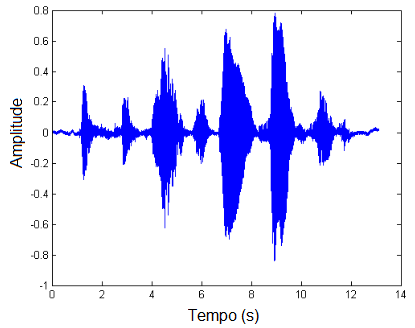
\includegraphics[width=0.75\textwidth]{imagens/exsinalsom.PNG}
\caption{\label{fig:exsinalsom}Exemplo de visualização de sinal sonoro, medindo a amplitude ao longo do tempo}

\author{Fonte: UNESP, Prinípios de Comunicações, 2013}
\end{figure}

\begin{figure}[!h]
\centering
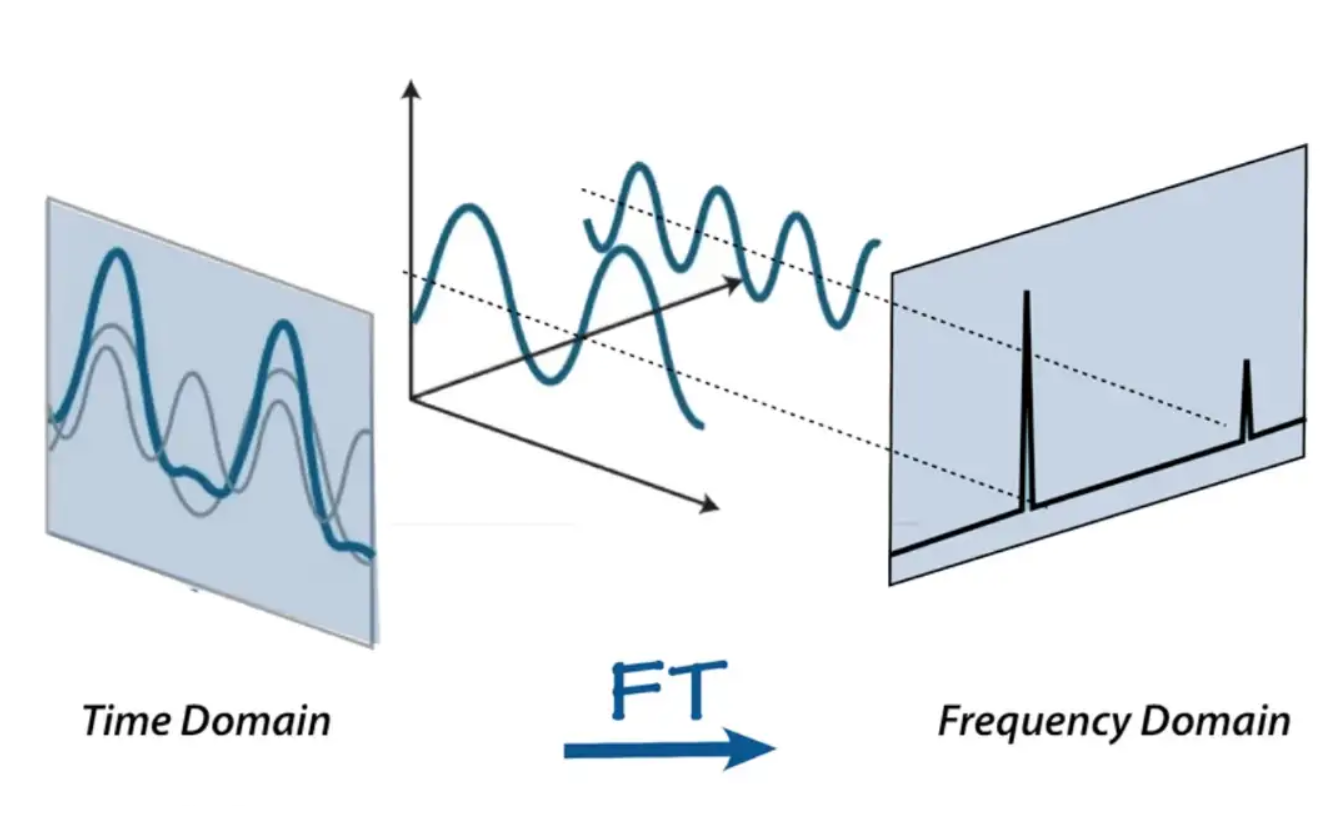
\includegraphics[width=0.6\textwidth]{imagens/ft.png}
\caption{\label{fig:fouriertransform}Ilustração da Transformada de Fourier}
\end{figure}

\clearpage

Com o resultado da \textit{FFT} de uma amostra, podemos calcular o seu espectrograma (\textit{spectrogram}): Uma representação da densidade das frequências ao longo do tempo. Entretanto, como humanos não compreendem todo o espectro sonoro \cite{62}, será aplicada uma normalização às frequências, e calcularemos o Espectrograma de Mel (\textit{Mel-Spectrogram}). Na Figura\footnote{Disponível em \url{https://medium.com/analytics-vidhya/understanding-the-mel-spectrogram-fca2afa2ce53}} \ref{fig:specvsmelespectrograma}, podemos observar a normalização das frequências (eixo vertical).

% https://towardsdatascience.com/learning-from-audio-the-mel-scale-mel-spectrograms-and-mel-frequency-cepstral-coefficients-f5752b6324a8
A normalização em questão, é a normalização pela escala de Mel (\textit{Mel Scale}). Uma escala construída para tornar tons equidistantes perceptivelmente equidistantes ao ouvido humano. A Escala de Mel é dada por:

\begin{equation}
    m(f) = 1127 * \log_e{(1 + \frac{f}{700})}
\end{equation}

\textit{Mel-Spectrogram} tem sido amplamente utilzada em problemas de \textit{SER}, como \cite{32.25} \cite{32.30}, e em \cite{32.31} e \cite{32.32}, que também utilizam \textit{CNN}s e ténicas de \textit{Autoencoder}.

Outro atributo observado na literatura são os Coeficientes Cepstrais de Frequência Mel (\textit{Mel Frequency Cepstral Coefficients}, \textit{MFCCs}). Um \textit{MFC} é uma representação de curto prazo do espectro de potência de um som, assim, \textit{MFC}s são os coeficientes que formam um \textit{MFCC} coletivamente. Calcular o \textit{MFCC} consiste em aplicar a Transformada Discreta do Cosseno (\textit{Discrete Cosine Transform}, \textit{DCT}) ao \textit{Mel-Spectrogram}. Podemos compreender o \textit{MFCC} como uma compressão \cite{64} do \textit{Mel Spectrogram}. Podemos observar um comparativo entre o resultado de um Mel-Spectrogram e um MFCC para uma mesma amostra na Figura \ref{fig:melspecvsmfcc}. Também encontramos trabalhos que utilizam \textit{MFCC}s em \cite{32.79} e \cite{32.89}, cujas arquiteturas contém uma CNN e uma GAN, respectivamente.

\clearpage

\begin{figure}[!h]
\centering
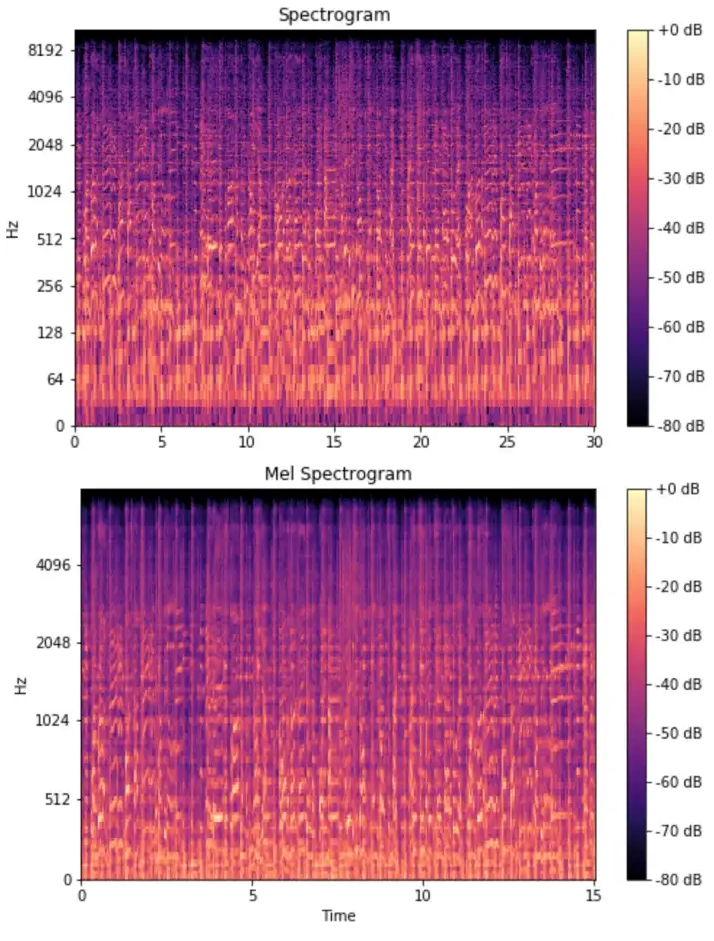
\includegraphics[width=0.55\textwidth]{imagens/espectrograma-vs-mel-espectrograma.png}
\caption{\label{fig:specvsmelespectrograma}Exemplos de Espectrograma e Espectrograma de Mel}
\end{figure}

\begin{figure}[!h]
\centering
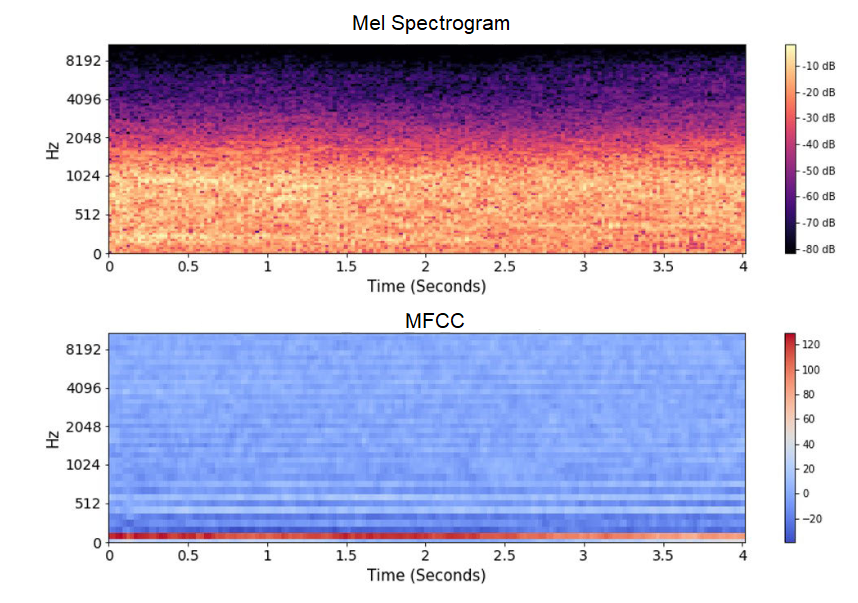
\includegraphics[width=0.7\textwidth]{imagens/melspec-vs-mfcc.PNG}
\caption{\label{fig:melspecvsmfcc}Espectrograma de Mel e MFCC de uma mesma amostra sonora}

\author{Fonte: Imagem adaptada de \cite{64}}
\end{figure}

% ==========================================================================================
\section{Métricas}\label{sec:metricas}

Na lista abaixo temos variáveis utilizadas para calcular as métricas de avaliação do desempenho de modelos de \textit{ML}:

\begin{itemize}
    \item Verdadeiros Positivos (VP) ou \textit{True Positive} (\textit{TP}): Classificação correta da classes positiva;
    \item Verdadeiros Negativos (VN) ou \textit{True Negative} (\textit{TN}): Classificação correta da classes negativa;
    \item Falsos Positivos (FP) ou \textit{False Positive} (\textit{FP}): Erro onde o modelo previu uma classe positiva, quando o valor real pertencia a classe negativa;
    \item Falsos Negativos (FN) ou \textit{False Negative} (\textit{FN}): Erro onde o modelo previu uma classe negativa, quando
o valor real pertencia a classe positiva.
\end{itemize}

Com essas variáveis, podemos calcular as seguintes métricas:

\begin{itemize}
    \item Acurácia (\textit{Accuracy}): Indica a performance geral do modelo.
        \begin{equation}
        \frac{VP + VN}{VP+FP+FN+FN}
        \end{equation}
    \item Precisão (\textit{Precision}): Dentre as classificações positivas que o modelo fez, quais foram corretas.
        \begin{equation}
        \frac{VP}{VP+FP}
        \end{equation}
    \item Sensibilidade (\textit{Recall}): Dentre todas as classificações positivas esperadas, quantas foram corretas.
        \begin{equation}
        \frac{VP}{VP+FN}
        \end{equation}
    \item \textit{F1-Score}: Média harmônica entre precisão e sensibilidade.
        \begin{equation}
        2 * \frac{precision  * recall}{precision + recall}
        \end{equation}
\end{itemize}

No âmbito de comparação de imagens, podemos citar o Índice de Similaridade Estrutural (\textit{Structural similarity}, \textit{SSIM}), que mede a similaridade entre duas imagens digitais. \textit{SSIM} é um modelo baseado na percepção, que considera a degradação da imagem como uma mudança percebida na sua informação estrutural, ao mesmo tempo em que incorpora fenômenos perceptivos de luminância e contraste, fornecendo um índice de qualidade para uma imagem (local). Tendo em vista o bom desempenho do sistema visual humano \cite{61} em perceber a estrutura visuais, o \textit{SSIM} se torna próximo da qualidade subjetiva que atribuimos a imagens.

O \textit{SSIM} é calculado em porções (janelas) da imagem, de modo que o índice entre duas janelas $x$ e $y$ de tamanho comum $NxN$ é dado por:

\begin{equation}
    % https://www.mathworks.com/help/images/ref/ssim.html
    SSIM(x,y) = [l(x,y)]^\alpha * [c(x,y)]^\beta * [s(x,y)]^\gamma
\end{equation}

Onde,

\begin{equation}
    l(x,y) = \frac{(2 * \mu_x * \mu_y) + C_1}{\mu_x^2 + \mu_y^2 + C_1}
\end{equation}

\begin{equation}
    c(x,y) = \frac{(2 * \sigma_x * \sigma_y) + C_2}{\sigma_x^2 + \sigma_y^2 + C_2}
\end{equation}

\begin{equation}
    s(x,y) = \frac{\sigma_{xy} + C_3}{(\sigma_x * \sigma_y) + C_3}
\end{equation}

E seus parâmetros, $\mu_x, \mu_y, \sigma_x, \sigma_y, \sigma_{xy}$, são as médias locais, desvios padrão e covariância cruzada para imagens $x, y$.

Quando $\alpha = \beta = \gamma = 1$ e $C3 = \frac{C2}{2}$, a equação fica simplificada da seguinte forma:

\begin{equation}
    SSIM(x,y) = \frac{(2 * \mu_x * \mu_y + C_1) * (2 * \sigma_{xy} + C_2)}{(\mu_x^2 + \mu_y^2 + C_1) * (\sigma_x^2 + \sigma_y^2 + C_2)}
\end{equation}


\chapter{Trabalhos Relacionados}\label{Cap:Trabalhos Relacionados}

Neste capítulo serão discutidos trabalhos relacionados e utilizados como referencial teórico por este material. Trataremos sobre suas propostas, características, metodologias, possíveis limitações e possibilidades de melhoria. Posteriormente, será feita uma análise comparativa com o trabalho proposto no Capítulo \ref{Cap:Projeto de Pesquisa}, evidenciando pontos em comum e possíveis divergências e, por fim, como este trabalho se propõe a colaborar com a produção científica e o estado da arte na área de \textit{SER}. Os trabalhos infracitados se encontram dispostos em ordem cronológica de publicação vide Tabela \ref{table:discussao}.\\

% ------------------------------------------------------------------------------------------

No âmbito das Ciências da Computação, o processamento de voz é uma área de pesquisa ativa, com publicações datando desde o final do século XX, podemos citar \cite{12.27} no ano de 1991 e \cite{12.28} em 1995.

% ------------------------------------------------------------------------------------------

Donn Morrison, Ruili Wang e Liyanage C. De Silva, em \textit{Ensemble methods for spoken emotion recognition in call-centres} \cite{32.32}, dada a ubuiquidade de sistems automatizados, lembram da necessidade de aprimorar a naturalidade das interações humano-computador e da importância de interpretar com precisão informações emocionais. Além de um \textit{dataset} tradicional (ESMBS), utilizou uma base de dados fornecida por uma companhia elétrica, composto por ligações de clientes para o \textit{call-center} da empresa, o que significa que não consistia de um \textit{dataset} simulado ou seminatural, e sim de uma massa de dados com amostras naturais e espontâneas. Afirma que um modelo de \textit{SER} pode colaborar com o atendimento aos clientes em chamadas de acordo com a urgência percebida. O que corrobora com este trabalho na importância, não só do diagnõstico da emoção, como também da sua intensidade. Caso seja detectada determinada emoção, o sistema transferiria a ligação para um atendente humano fornecer assistência. Entretanto, mesmo com a combinação de duas massas de dados, o dataset final contava com pouco mais de mil amostras (1100), sendo 93\% pertencente a classe neutra. Quanto aos algoritmos, foram utilzados dez modelos tradicionais (\textit{SVM radial basis}, \textit{KNN}, \textit{MLP}, \textit{RF}, \textit{K*}, \textit{NAIVE BAYES}, \textit{SVM polinomial}, \textit{Decision Tree e Random Tree}), combinados em forma de ensemble, sem pesos individuais, para realizar a predição, alcançando acurácia média (72,18\%) ligeiramente superior aos modelos individuais.

Mayank Bhargava e Tim Polzehl, em \textit{Improving Automatic Emotion Recognition from speech using Rhythm and Temporal feature} \cite{11}, se propõem a melhorar o desempenho em tarefas de \textit{SER} incorporando mais features aos dados de entrada. Aponta que pesquisas à época dependiam fortemente de \textit{MFCCs}, tonalidade e da amplitude. Dicidiu utilizar um algoritmo (\textit{Voice Activity Detection}, \textit{VAD}) para separar, a nível de amostra, os momentos com linguagem presente, e performar a extração de características separadamente. Validou sua abordagem com dois modelos, um \textit{DNN} e um \textit{SVM}, ao longo de sete classes. Apesar dos modelos, o escopo do trabalho seria o de relacionar a melhora no desempenho dos modelos com a adição ou combinação de mais features, entretanto, observou que os melhores resultados de índice de acerto foram obtidos em dois cenários: (1) 74.02\% utilizando \textit{MFCCs} e características rítmicas, embora o resultado utilizando apenas features rítmicas fosse de apenas 34.6\%; e (2) 71.93\% utilizando apenas \textit{MFCCs}. Sobre as características rítmicas, ressaltou que sua baixa contribuição dá-se possivelmente em virtude da baixa dimensionalidade, uma vez que é mais de dez vezes menor que a dos MFCCs. Os resultados de \cite{11} foram, de certa forma, contrários a sua hipótese, e reasseguraram a eficiência de utilizar features espectrográficas para tarefas de SER.

Xiaoming Zhao e Shiqing Zhang, em\textit{ Spoken emotion recognition via locality-constrained kernel sparse representation }\cite{32.31}, propõem um método para classificação de emoções denominado \textit{locality-constrained kernel sparse representation-based classification} (\textit{LC-KSRC}), capaz de aprender com representações de coeficientes mais esparsas, utilizando features prosódicas, espectrais e de qualidade da voz. Uma vez que a localidade dos dados tem tem sido amplamente utilizada em muitos problemas de reconhecimento de padrões como \textit{clustering}, \textit{dimensionality reduction} e classificação de imagens, \cite{32.31} combina as técnicas \textit{Sparse representation-based classification} (\textit{SRC}), \textit{Kernel sparse representation-based classification} (\textit{KRSC}) e \textit{Locality-constrained linear coding} (\textit{LLC}) para formar \textit{LC-KSRC} e tentar compor sobre o problema de perda de captura da estrutura dados locais de \textit{KRSC}. Testado em quatro bases de dados distitnas, o modelo proposto apresenteu acurária superior a todos os outros seis modelos com o qual foi comparado. Xiaoming Zhao e Shiqing Zhang apontam para a o desafio de produzir soluções de SER que atuem em tempo real.

Sonia Xylina Mashal e Kavita Asnani, em\textit{ Emotion Intensity Detection for Social Media Data }\cite{14}, observam que embora sejam desenvolvidos trabalhos na área de reconhecimento de emoções, essa classificação é um resultado de mais rudimentar, e o próximo passo seria determinar a intensidade dessa emoção. Portanto, investigaram um classificador para determinar a intensidade das emoções em textos, utilizando dados obtidos a partir de uma base de dados formada por textos do Twitter. As amostras eram compostas por textos curtos (tweets) e um valor entre 0 e 1 relativo a intensidade da emoção sentida pelo autor.

Zhang, S. et al., em \textit{Speech Emotion Recognition Using Deep Convolutional Neural Network and Discriminant Temporal Pyramid Matching} \cite{32.25}, aponta o distanciamento entre as emoções, subjetivas, e as features de baixo nível. Observa o bom desempenho de \textit{CNNs} em tarefas de reconhecimento de imagem e detecção de objeto e explora como utilizar essas redes para tentar encurtar essa distância. De maneira análoga ao que é feito em tarefas que envolvem imagens, extraindo os três canais correspondentes as cores vermelho, verde e azul (red, green e blue, respectivamente, formando a sigla \textit{RGB}), este, a partir do \textit{Mel Spectrogram} da amostra, extrai três canais: Estático (\textit{static}), delta, e delta delta. Para realizar \textit{feature extraction}, utiliza a \textit{CNN} \textit{AlexNET}, uma rede neural pré-treinada para reconhecimento de imagens, para tentar aprender características de alto nível a respeito das vocalizações. Propõe então uma \textit{Discriminant Temporal Pyramid Matching} (\textit{DTPM}), inspirado na \textit{Spatial Pyramid Matching} (\textit{SPM}), para agrupar as features aprendidas em uma unidade maior e aplicando um modelo \textit{SVM} linear na nesse resultado. Embora tenha utilizado mais de um dataset em sua tarefa, \cite{32.25} aponta a quantidade limitada de amostras disponíveis para treinamento e afirma que o modelo AlexNET apresenta um bom desempenho na tarefa de feature extracion.

Sefik Emre Eskimez, Zhiyao Duan e Wendi Heinzelman, em \textit{UNSUPERVISED LEARNING APPROACH TO FEATURE ANALYSIS FOR AUTOMATIC SPEECH EMOTION RECOGNITION} \cite{34}, propõem a utilização de modelos não supervisionados do tipo autoencoder, separadamente, para tentar remediar a escassez de dados para tarefas de \textit{SER}, questionando a viabilidade de aprendender \textit{features} de \textit{datasets} de outros domínios de voz e utilizá-los para treinar modelos de classificação de emoções. Os modelos não supervisionados incluem\textit{ Denoising Autoencoder} (\textit{DAE}), \textit{Variational Autoencoder} (\textit{VAE}), \textit{Adversarial Autoencoder} (\textit{AAE}) e \textit{Adversarial Variational Baye}s (\textit{AVB}) com adição de ruído. Utilizou um \textit{SVM} e \textit{CNN} como modelos de base para avaliar o desempenho dos \textit{autoencoders}. Os modelos receberam\textit{ Mel Spectrograms} para efetuar a classificação das emoções, e \cite{34} chegou a conclusão de que os modelos inferenciais (\textit{VAE}, \textit{AAE} e \textit{AVB}) obtiveram um desempenho superior tarefa de aprendizado não supervisionado de aprendizado de features.

Yuanchao Li, Tianyu Zhao e Tatsuya Kawahara, em \textit{Improved End-to-End Speech Emotion Recognition Using Self Attention Mechanism and Multitask Learning} \cite{32.95}, propõem um modelo \textit{multitask} utilizando uma camada de autoatenção (\textit{self attention layer}) para classificar tanto a emoção quanto o sexo da pessoa, apesar das dificuldades em virtude da variabilidade em dados de fala e emoção. Utiliza os espectrogramas como \textit{input} para um modelo composto por uma CNN\textit{ }que alimenta uma \textit{BLSTM} seguida pela camada de autoatenção para agregar informações da camada anterior ao longo do tempo. Utilizando a base de dados IEMOCAP, afirmou ter superado (à época, 2019) os melhores resultados de classificação relativos ao dataset.

M. S. Akhtar et al., em \textit{All-in-One: Emotion, Sentiment and Intensity Prediction using a Multi-task Ensemble Framework} \cite{28}, propõe um \textit{ensemble} de modelos para a multitarefa de classificar emoção e intensidade em texto. Utilizando 3 modelos para feature extraction (\textit{\textit{CNN, \textit{LSTM} e GRU}}) e processamento de linguagem natural (\textit{NLP}) para adicionar mais uma dimensão ao vetor de entrada, observa que modelos multitarefa constumam ter desempenhos superiores em matéria de generalização. As bases de dados utilizadas apresentavam as emoções como classe, e a intensidade foi calculada a partir da técnica de Vader\footnote{Disponível em \url{https://ojs.aaai.org/index.php/ICWSM/article/view/14550}}. Akhtar avaliou tanto o desempenho dos modelos individuais quanto combinações (\textit{ensembles}) para concluir que os \textit{ensembles} propostos apresentaram desempenho superior aos modelos individuais.

Zhu et al., em\textit{ Controlling Emotion Strength with Relative Attribute for End-to-End Speech Synthesis} \cite{63}, pretende melhorar a performance da síntese de uma vocalização emocional oriunda de um mecanismo de conversão de texto para fala (\textit{speech to text}, \textit{STT}). Focando apenas no controle sutil da intensidade da emoção, simplificando o controle da emoção e da intensidade através de um vetor e um escalar, respectivamente, para que consgiga modular com facilidade a itensidade de uma amostra. A base de dados utilizada é composta por várias sentenças que são repetidas tendo sua classe (emoção) alterada. Embora não possua labels para a intensidade, \cite{63} busca calcular uma função de ranqueamento de atributo (\textit{attribute ranking function}) entre pares formados por classes distintas de uma mesma amostra e utilizar esse atributo em combinação com uma amostra de uma classe para produzir a amostra pertencente outra classe, de acordo com o atributo. Uma vez calculada a \textit{ranking function}, um algoritmo não supervisionado de redução de dimensionalidade (\textit{PCA}) foi aplicado numa amostra da base de dados, onde foi observada a coerência entre as classes de dados dados de um mesmo conjunto (\textit{cluster}).

Aggelina Chatziagapi et al., em \textit{Data Augmentation using GANs for Speech Emotion Recognition }\cite{32.89}, propõem um modelo de \textit{GAN} para atacar o problema de conjuntos de dados desbalanceados em tarefas de \textit{SER}. Fato que podemos observar em \cite{32.32} e soma-se a um ponto descrito nesse trabalho, sobre a discrepância em volume de dados para tarefas de \textit{SER} com realação a outras tarefas, como reconhecimento de imagens, e mais ainda no contexto de intensidade das emoções. Busca produzir novas amostras de spectrogramas para classes menos representadas. Embora não seja propriamente uma proposta para reconhecimento de emoções ou de intensidade das emoções, \cite{32.89} utiliza duas bases de dados, IEMOCAP e FEEL-25k, para validar o resultado do seu modelo. Uma vez que os spectrogramas gerados artificialmente são incluídos ao conjunto do dataset, calcula a distribuição das classes, e então passa a retirar amostras aleatoriamente, observando que as porcentagens das classes se mantém equilibrada ao longo da remoções.

Campos e Moutinho, em DEEP: Uma arquitetura para reconhecer emoção com base no espectro sonoro da voz de falantes da língua portuguesa \cite{12}, se propõem a criar um modelo mais robusto, com uma implementação híbrida. Observaram que a utilização de múltiplas redes neurais de maneira sequencial pode ocasionar a propagação de erros entre os modelos. Assim, seu modelo é composto por vários modelos especialistas, que combinam redes neurais convolucionais e redes neurais profundas, treinados de forma supervisionada. Campos e Coutinho treinaram um modelo especialita para cada uma das sete emoções presentes no dataset VERBO. Além de reiterar a usabilidade da base de dados, tiveram ganhos em sua taxa média de acerto acima de 10\% quando comparando sua implementação com uma CNN simples.

Neelakshi Josh, em \textit{Brazilian Portuguese emotional speech corpus analysis} \cite{20}, se propôs a explorar diferentes features de um banco de dados em poruguês brasileiro. Procurou explorar características espectrais, prosódicas e temporais numa tarefa de SER, afirmando que a utilização conjunta dessas características podem melhorar o seu índice de acerto. Totalizando 38 \textit{features} em um vetor, treinou quatro algoritmos, utilizando apenas a abordagem supervisionada: \textit{SVM}, \textit{MLP},\textit{RF} e \textit{KNN}. Utilizou a base de dados VERBO, também utilizada neste trabalho, colaborando com a evidência de que apesar de ser o primeiro dataset para SER em português brasileiro, este pode ser utilizado para trabalhos de \textit{SER} e que suas amostras possuem características suficientes para desenvolver tarefas de \textit{ML}. Embora tenha utilizado quatro modelos distintos, Neelakshi não se aprofundou em demais arquiteturas de \textit{Deep Learning}.

Abbaschian, Sierra-Sosa e Elmaghraby, em \textit{Deep Learning Techniques for Speech Emotion Recognition from Databases to Models} \cite{32}, revisam publicações que envolvem trabalhos de \textit{Deep Learning} para \textit{SER}, bem como as bases de dados utilizadas. Realiza um comparativo entre onze bases de dados amplamente utilizadas em trabalhos dessa natureza, dispostas em três categorias: Simuladas, seminaturais e naturais. Realizam um cruzamento entre 25 databases e trabalhos que as utilizam, organizando essa relação ao longo do tempo, disposto num eixo horizontal que compreende os anos entre 2005 e 2020. Nessa relação podemos perceber a predominância de certos entes em determinados períodos do tempo, tanto com relação a datasets quanto a modelos. Quanto as bases de dados, a partir de 2018 percebemos a predominância do IEMOCAP, sendo utilizado o dobro de vezes em relação ao EMO-DB, segundo mais utilizado. Quanto aos modelos, percebemos a presença constante de \textit{CNNs} a partir de 2016 e de variações de \textit{Autoencoders} a partir de 2018, ambos permanecendo presentes até 2020, ano final da cobertura da pesquisa.

% \cite{18}-2022
Kun Zhou et al., em \textit{Emotion Intensity and its Control for Emotional Voice Conversion }\cite{18}, comenta a parca presença de estudos relativos a intensidade da emoção, uma vez que têm um grande potencial para a conversão de voz. O trabalho consistem em conseguir controlar a intensidade da emoção em um modelo de sequência para sequência (\textit{seq2seq}) que converte texto para voz. De maneira análoga a \cite{63}, Zhou também decide encontrar uma \textit{attribute ranking function} para operar com o dado de entrada e alterar a intensidade da emoção da maneira desejada. Kun \cite{18} e Zhu \cite{63} diferem na sua arquitetura, enquanto \cite{63} utiliza um \textit{autoencoder} que recebe o escalar relativo a intensidade após a fase de \textit{encoding}, \cite{18} utiliza três modelos com funções disntantas: (1) Extrair as features do \textit{input}; (2) Criar adicionar a emoção desejada para a saída; e (3) Adicionar a alteração na intensidade.

% ==========================================================================================
\section{Discussão dos Trabalhos Relacionados}

Conseguimos observar nos trabalhos supracitados que dificuldades relativas à massa de dados não é um problema exclusivo de trabalhos em SER, uma vez que os trabalhos que lidam dados textuais reiteram essa queixa, sejam os que lidam puramente com textos ou os que realizam tarefas de \textit{text-to-speach} com emoção.

Ainda no ano de de 2007, \cite{32.32} lembrou da ubiquidade de sistemas automatizados, que se mostra ainda mais presente contemporaneamente. Ao efetuarmos um comparativo (Tabela \ref{table:discussao}) entre trabalhos com tarefas de reconhecimento de emoções na fala, vemos que apesar de \cite{14} afirmar que a atividade de classificaçar emoções poderia ter um papel adicional enquanto catalisador para trabalhos envolvendo a intensidade da emoção, no entantdo, a incidência de trabalhos nessa área específica parece baixa.

A subjetividade das emoções demanda cuidado e atuação profissional na composição de bancos de dados para esse tipo de tarefa. Ao reduzir o escopo da pesquisa para trabalhos com dados em português, a literatura se torna ainda mais escassa, haja vista a publicação do VERBO apenas no ano de 2018.

Características espectrais aparentam ser uma feature importante para os modelos, carregadando bastante informacional sobre a amostra. Pudemos observar em \cite{11} que a ausência de \textit{MFCCs} acarretou uma queda superior a 50\% na performance da classificação, enquanto \cite{34} os utilizou como \textit{target} para redes generativas enquanto buscava aumentar a quantidade de amostrass disponíveis para treinamento de modelos.

Outro ponto a ser observado é que embora existam trabalhos utilizando mais de um \textit{dataset}, essa prática ainda não parece estar totalmente difundida entre as publicações de \textit{SER}, uma vez que os escopos e naturezas (simulada, seminatural ou natural) das bases de dados costumam ser bastante distintas.

Analisando as informações expostas na Tabela \ref{table:discussao}, podemos notar que estre trabalho se aproxima dos demais por utilizar features espectrais e envolver uma abordagem supervisionada. Também tem em comum o fato de utilzar técnicas consolidadas ("clássicas") de \textit{ML}, ao mesmo tempo que investiga arquiteturas de \textit{DL}, como DNNs, \textit{CNNs} e \textit{Autoencoders}. Entretanto, este trabalho começa a se distanciar dos demais quando resolver trabalhar com áudios para a língua portuguesa. Além disso, a abordagem não supervisionadas também será utilizada, o que não é tão comum em uma mesma tarefa de \textit{SER}. Outro ponto de inovação dá-se uma vez que os trabalhos que encontramos utilzando o dataset VERBO têm apenas utilizaram apenas aprendizagem supervisionado e não lidam com intensidade. Ademais, não foram encontrados trabalhos utilizando o dataset VIVAE (2020), possivelmente tornando este trabalho pioneiro.

% \clearpage

% -------------------------------------------------------------------------------------------

% ~~~~~~~~~~~~~~~~~~~~~~~~~~~~~~~~~~~~~~~~~~~
% gerada em https://www.tablesgenerator.com/
% ~~~~~~~~~~~~~~~~~~~~~~~~~~~~~~~~~~~~~~~~~~~

\begin{landscape}
\begin{table}[]
\centering
\label{table:discussao}
\caption{Comparativo entre BRAVO e literatura correlata}
\begin{tabular}{|
>{\columncolor[HTML]{FFFFFF}}c |
>{\columncolor[HTML]{FFFFFF}}l |
>{\columncolor[HTML]{FFFFFF}}c 
>{\columncolor[HTML]{FFFFFF}}c 
>{\columncolor[HTML]{FFFFFF}}c |
>{\columncolor[HTML]{FFFFFF}}c 
>{\columncolor[HTML]{FFFFFF}}c |
>{\columncolor[HTML]{FFFFFF}}c 
>{\columncolor[HTML]{FFFFFF}}c |
>{\columncolor[HTML]{FFFFFF}}c 
>{\columncolor[HTML]{FFFFFF}}c |
>{\columncolor[HTML]{FFFFFF}}c 
>{\columncolor[HTML]{FFFFFF}}c |}
\hline
\cellcolor[HTML]{FFFFFF} & \multicolumn{1}{c|}{\cellcolor[HTML]{FFFFFF}} & \multicolumn{3}{c|}{\cellcolor[HTML]{FFFFFF}Features} & \multicolumn{2}{c|}{\cellcolor[HTML]{FFFFFF}Abordagem} & \multicolumn{2}{c|}{\cellcolor[HTML]{FFFFFF}Arquitetura} & \multicolumn{2}{c|}{\cellcolor[HTML]{FFFFFF}Português} & \multicolumn{2}{c|}{\cellcolor[HTML]{FFFFFF}Resultado} \\ \cline{3-13} 
\multirow{-2}{*}{\cellcolor[HTML]{FFFFFF}ANO} & \multicolumn{1}{c|}{\multirow{-2}{*}{\cellcolor[HTML]{FFFFFF}Referência}} & \multicolumn{1}{c|}{\cellcolor[HTML]{FFFFFF}Cromática} & \multicolumn{1}{c|}{\cellcolor[HTML]{FFFFFF}Espectral} & Prosódica & \multicolumn{1}{c|}{\cellcolor[HTML]{FFFFFF}Superv.} & Não superv.& \multicolumn{1}{c|}{\cellcolor[HTML]{FFFFFF}ML} & DL & \multicolumn{1}{c|}{\cellcolor[HTML]{FFFFFF}Não} & Sim & \multicolumn{1}{c|}{\cellcolor[HTML]{FFFFFF}Emoção} & Intensidade \\ \hline
% 1995 & {\cite{12.28}} & \multicolumn{1}{c|}{\cellcolor[HTML]{FFFFFF}} & \multicolumn{1}{c|}{\cellcolor[HTML]{FFFFFF}} & X & \multicolumn{1}{c|}{\cellcolor[HTML]{FFFFFF}} &  & \multicolumn{1}{c|}{\cellcolor[HTML]{FFFFFF}X} &  & \multicolumn{1}{c|}{\cellcolor[HTML]{FFFFFF}X} &  & \multicolumn{1}{c|}{\cellcolor[HTML]{FFFFFF}} &  \\ \hline
2007 & {\cite{32.32}} & \multicolumn{1}{c|}{\cellcolor[HTML]{FFFFFF}} & \multicolumn{1}{c|}{\cellcolor[HTML]{FFFFFF}} & X & \multicolumn{1}{c|}{\cellcolor[HTML]{FFFFFF}X} &  & \multicolumn{1}{c|}{\cellcolor[HTML]{FFFFFF}X} &  & \multicolumn{1}{c|}{\cellcolor[HTML]{FFFFFF}X} &  & \multicolumn{1}{c|}{\cellcolor[HTML]{FFFFFF}X} &  \\ \hline
2013 & {\cite{11}} & \multicolumn{1}{c|}{\cellcolor[HTML]{FFFFFF}} & \multicolumn{1}{c|}{\cellcolor[HTML]{FFFFFF}X} & X & \multicolumn{1}{c|}{\cellcolor[HTML]{FFFFFF}X} &  & \multicolumn{1}{c|}{\cellcolor[HTML]{FFFFFF}X} & X & \multicolumn{1}{c|}{\cellcolor[HTML]{FFFFFF}X} &  & \multicolumn{1}{c|}{\cellcolor[HTML]{FFFFFF}} &  \\ \hline
2015 & {\cite{32.31}} & \multicolumn{1}{c|}{\cellcolor[HTML]{FFFFFF}X} & \multicolumn{1}{c|}{\cellcolor[HTML]{FFFFFF}X} & X & \multicolumn{1}{c|}{\cellcolor[HTML]{FFFFFF}X} &  & \multicolumn{1}{c|}{\cellcolor[HTML]{FFFFFF}} & X & \multicolumn{1}{c|}{\cellcolor[HTML]{FFFFFF}X} &  & \multicolumn{1}{c|}{\cellcolor[HTML]{FFFFFF}X} &  \\ \hline
2018 & {\cite{32.25}} & \multicolumn{1}{c|}{\cellcolor[HTML]{FFFFFF}} & \multicolumn{1}{c|}{\cellcolor[HTML]{FFFFFF}X} &  & \multicolumn{1}{c|}{\cellcolor[HTML]{FFFFFF}X} &  & \multicolumn{1}{c|}{\cellcolor[HTML]{FFFFFF}X} &  & \multicolumn{1}{c|}{\cellcolor[HTML]{FFFFFF}X} &  & \multicolumn{1}{c|}{\cellcolor[HTML]{FFFFFF}X} &  \\ \hline
2018 & {\cite{34}} & \multicolumn{1}{c|}{\cellcolor[HTML]{FFFFFF}} & \multicolumn{1}{c|}{\cellcolor[HTML]{FFFFFF}X} &  & \multicolumn{1}{c|}{\cellcolor[HTML]{FFFFFF}X} & X & \multicolumn{1}{c|}{\cellcolor[HTML]{FFFFFF}} & X & \multicolumn{1}{c|}{\cellcolor[HTML]{FFFFFF}X} &  & \multicolumn{1}{c|}{\cellcolor[HTML]{FFFFFF}X} &  \\ \hline
2019 & {\cite{32.95}} & \multicolumn{1}{c|}{\cellcolor[HTML]{FFFFFF}} & \multicolumn{1}{c|}{\cellcolor[HTML]{FFFFFF}X} &  & \multicolumn{1}{c|}{\cellcolor[HTML]{FFFFFF}X} &  & \multicolumn{1}{c|}{\cellcolor[HTML]{FFFFFF}} & X & \multicolumn{1}{c|}{\cellcolor[HTML]{FFFFFF}X} &  & \multicolumn{1}{c|}{\cellcolor[HTML]{FFFFFF}X} &  \\ \hline
2020 & {\cite{12}} & \multicolumn{1}{c|}{\cellcolor[HTML]{FFFFFF}X} & \multicolumn{1}{c|}{\cellcolor[HTML]{FFFFFF}X} & X & \multicolumn{1}{c|}{\cellcolor[HTML]{FFFFFF}X} &  & \multicolumn{1}{c|}{\cellcolor[HTML]{FFFFFF}} &  & \multicolumn{1}{c|}{\cellcolor[HTML]{FFFFFF}} & X & \multicolumn{1}{c|}{\cellcolor[HTML]{FFFFFF}X} &  \\ \hline
2021 & {\cite{21}} & \multicolumn{1}{c|}{\cellcolor[HTML]{FFFFFF}X} & \multicolumn{1}{c|}{\cellcolor[HTML]{FFFFFF}X} & X & \multicolumn{1}{c|}{\cellcolor[HTML]{FFFFFF}X} &  & \multicolumn{1}{c|}{\cellcolor[HTML]{FFFFFF}X} & X & \multicolumn{1}{c|}{\cellcolor[HTML]{FFFFFF}} & X & \multicolumn{1}{c|}{\cellcolor[HTML]{FFFFFF}X} &  \\ \hline
\textit{\textbf{2023}} & \textit{\textbf{BRAVO}} & \multicolumn{1}{c|}{\cellcolor[HTML]{FFFFFF}\textit{\textbf{}}} & \multicolumn{1}{c|}{\cellcolor[HTML]{FFFFFF}\textit{\textbf{X}}} & \textit{\textbf{}} & \multicolumn{1}{c|}{\cellcolor[HTML]{FFFFFF}\textit{\textbf{X}}} & \textit{\textbf{X}} & \multicolumn{1}{c|}{\cellcolor[HTML]{FFFFFF}\textit{\textbf{X}}} & \textit{\textbf{X}} & \multicolumn{1}{c|}{\cellcolor[HTML]{FFFFFF}\textit{\textbf{}}} & \textit{\textbf{X}} & \multicolumn{1}{c|}{\cellcolor[HTML]{FFFFFF}\textit{\textbf{}}} & \textit{\textbf{X}} \\ \hline
\end{tabular}
\end{table}
\end{landscape}

\chapter{Projeto de Pesquisa}\label{Cap:Projeto de Pesquisa}

Neste capítulo é apresentada a proposta contida neste trabalho. O capítulo irá se desdobrar a partir do problema encontrado e proporá uma solução para sua realização. Adiante, irá expor a sua implementação em detalhes, tratando conhecimentos mais específicos que não estejam elucidados ao longo dos capítulos anteriores e conjecturando sobre possíveis aplicabilidades deste trabalho em áreas diversas. Finalmente, as atividades propostas para este projeto de pesquisa, juntamente com um cronograma de acompanhamento, de acordo com o estabelecido pelo Programa de Pós-Graduação em Informática da Universidade de Brasília (PPGI/UnB) para a obtenção do título de Mestre.\\

% ==========================================================================================
\section{Motivação}

Independente de formação enquanto profissionais de saúde mental, é natural que consigamos atribuir alguma espécie de métrica para comparar duas instâncias de uma mesma emoção que tenhamos sentido. Parece trivial quando atestamos que, entre dois momentos experimentando uma mesma emoção, um foi mais ou menos intenso do que o outro, ou até que ambos tiveram a mesma intensidade. Portanto, somos capazes de identificar emoções, quantificar sua intensidade e calcular uma distância para poder efetuar essa comparação.

Conforme visto, trabalhos de \textit{ML} aplicados ao reconhecimento de emoções na fala vêm sendo publicados - ao menos - desde o início da década de 90 (1990), e se tornam menos frequentes quando buscamos por tarefas mais especializadas.

Não tendo encontrado ocorrência na literatura, este trabalho se propõe a responder a seguinte pergunta: É possível realizar uma tarefa de aprendizado de máquina para inferir a intensidade das emoções na voz em português?

% ==========================================================================================
\section{\textit{BRAVO: Brazilian-portuguese Emotional Intensity Recognition Assistant for Voice}}

% ------------------------------------------------------------------------------------------
\subsection{Visão Geral}

Na Figura \ref{fig:visaogeralproposta} é apresentada uma visão geral da proposta. Conforme a imagem, três etapas principais serão necessárias para o reconhecimento da intensidade das emoções: (A) Aquisição dos dados; (B) Extração de características; e (C) Classificação da intensidade.

\begin{figure}[!h]
\centering
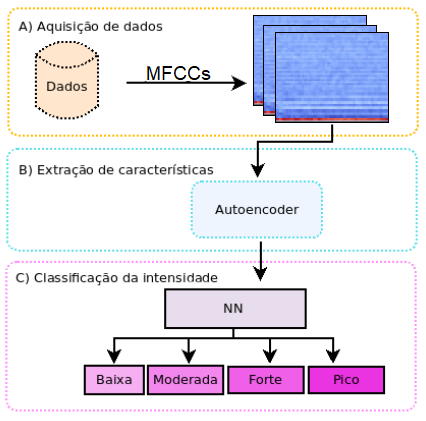
\includegraphics[width=0.75\textwidth]{imagens/arquitetura-visao-geral-2.png}
\caption{\label{fig:visaogeralproposta}Visão geral da proposta}
\end{figure}

A primeira etapa (A) lida com a obtenção dos dados que serão utilizados no projeto e da sua conversão para uma interpretação passível de utilização por modelos de aprendizagem de máquina. Podemos descrever os dados como um conjunto de registros rotulados que serão utilizados para treinamento, teste e validação dos modelos implementados na proposta.

A segunda etapa (B) lida com a extração de características dos dados convertidos. Essas \textit{features} serão obtidas através de um modelo não supervisionado para a redução de dimensionalidade e posteriormente utilizadas como entrada de um modelo supervisionado de classificação da intensidade da emoção.

A terceira e última etapa (C) é responsável pela inferência da intensidade. O modelo recebe as \textit{features} obtidas na etapa anterior e realiza o treinamento e testagem do modelo de classificação de acordo com quatro classes possíveis: (i) Baixa; (ii) Moderada; (iii) Forte; e (iv) Pico de intensidade.

% ------------------------------------------------------------------------------------------
\subsection{Aquisição dos dados}

O primeiro passo para tarefas de \textit{machine learning} que envolvem \textit{SER} costuma ser a aquisição dos dados que serão utilizados pelo modelo. Em virtude do escopo da proposta, necessitamos de um \textit{dataset} em português que possua as classes desejadas: Emoção e intensidade.

Até o momento da escrita deste tabalho, não sabemos de nenhum \textit{dataset} que seja ideal (idioma, emoções e intensidade) para esta proposta. Então, conforme descrito na seção \ref{section:basesdedados}, este trabalho utilizará duas bases de dados: VERBO \cite{12.21} e VIVAE \cite{16}.

O primeiro \textit{dataset}, VERBO, é composto por vocalizações verbais, acomodando todos os fonemas da língua portuguesa, com exemplos para seis emoções básicas (alegria, nojo, medo, raiva, surpresa, tristeza) e um estado emocional denominado de neutro.

O segundo, VIVAE, é composto por vocalizações não verbais distribuidas em seis classes (conquista, prazer sexual, surpresa positiva, raiva, medo e dor física), com exemplos em quatro intensidades (baixa, moderada, fote e pico de intensidade). Graças a fusão de domínios \cite{49}, conseguimos o cenário da Tabela \ref{table:datasetideal}.

Assim, sejam os dois \textit{datasets} VERBO e VIVAE, de modo que VERBO é constituído por pares \{amostra, classe\} e VIVAE por pares \{amostra, classe, intensidade\}, onde as classes são a emoção atribuída àquela amostra, e a intensidade é o rótulo da intensidade da classe daquela amostra. Vamos representar as amostras do VERBO por $X_{VERBO}$ e do VIVAE por $X_{VIVAE}$.

\begin{table}[!h]
\centering
\label{table:datasetideal}
\caption{Atributos dos datasets VERBO, VIVAE, ideal e da fusão de domínios}
\begin{tabular}{l|cccc|}
\cline{2-5}
 & \multicolumn{4}{c|}{Datasets} \\ \hline
\multicolumn{1}{|l|}{Atributos} & \multicolumn{1}{c|}{VERBO} & \multicolumn{1}{c|}{VIVAE} & \multicolumn{1}{c|}{Ideal} & Data Fusion(VERBO,VIVAE) \\ \hline
\multicolumn{1}{|l|}{Idioma} & \multicolumn{1}{c|}{X} & \multicolumn{1}{c|}{} & \multicolumn{1}{c|}{X} & X \\ \hline
\multicolumn{1}{|l|}{Emoções} & \multicolumn{1}{c|}{X} & \multicolumn{1}{c|}{X} & \multicolumn{1}{c|}{X} & X \\ \hline
\multicolumn{1}{|l|}{Intensidade} & \multicolumn{1}{c|}{} & \multicolumn{1}{c|}{X} & \multicolumn{1}{c|}{X} & X \\ \hline
\end{tabular}
\end{table}

Seja $Y_{VERBO}$ o conjunto das classes (emoções) $y_i \forall x_i \in X_{VERBO}$, analogamente para $Y_{VIVAE}$, vamos definir $Y = Y_{VERBO} \bigcap Y_{VIVAE}$. Vamos definir por por $Z$ o conjunto das intensidades. Sabemos das Tabelas \ref{table:vivaeintensidade} e \ref{table:totalporclasse} que

\begin{itemize}
    \item $Y = \{alegria, medo, raiva, supresa\}$
    \item $Z = \{baixa, moderada, forte, pico\}$
\end{itemize}

\begin{figure}[!h]
\centering
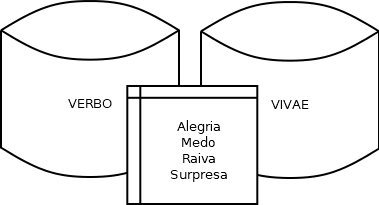
\includegraphics[width=0.40\textwidth]{imagens/p-yverbointeryvivae.png}
\caption{\label{fig:yverbointeryvivae}Interseção entre rótulos de emoções de VERBO e VIVAE}
\end{figure}

Vamos redefinir $X_{VERBO} = \{x_i \mid y_i \in Y\}$, analogamente para $X_{VIVAE}$, e vamos definir nosso domínio $X = X_{VERBO} \bigcap X_{VIVAE}$, assim

\begin{itemize}
    \item $\forall x_i \in X, \exists y_i \in Y$ tal que  $y_i$ é a classe de $x_i$
    \item $\forall x_j \in X_{VIVAE}, \exists z_j \in Z$ tal que  $z_j$ é a intensidade de $x_j$
\end{itemize}

Ao realizar tarefas de \textit{DL}, precisamos transformar os dados de entrada em um formato passível de ingestão pelos modelos. Os arquivos \textit{.wav} de $X$ serão lidos e iremos gerar seus respectivos \textit{MFCCs}, convertendo o sinal de áudio ao longo do tempo para uma representação do sinal no domínio da frequência, que será utilizada pelos modelos. Então, teremos um mapa $M(x_i): MFCC_i$.

\begin{figure}[!h]
\centering
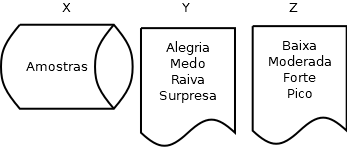
\includegraphics[width=0.5\textwidth]{imagens/p-dominios-contradominos.png}
\caption{\label{fig:dominioscontradominios}Domínio e contradomínios}
\end{figure}

% ------------------------------------------------------------------------------------------
\subsection{Extração de características}

De posse do mapa $M(x_i)$, podemos prosseguir para a etapa de extração de características. Apesar da representação visual, o espectrograma é dado por um vetor de alta dimensionalidade. Uma vez que $X$ é formado por dados de \textit{datasets} diferentes, buscamos uma forma de extrair características relevantes com boa capacidade de generalização ao ser aplicada em ambos $X_{VERBO}$ e $X_{VIVAE}$.

Redes neurais constituem uma boa ferramenta para tarefas de \textit{SER}. CNNs como \textit{feature extractors}, mais ainda \textit{Autoencoders}, podem criar uma representação de qualidade com dimensionalidade reduzida em seu espaço latente, enquanto \textit{DNNs} encotram espaço na literatura como bons discriminadores ou classificadores.

Vamos construir um \textit{Autoencoder} ($AE$) que tenta reproduzir uma função identendide. Por definição, um \textit{Autoencoder} é composto por uma função \textit{encoder} ($f_e$) e uma função $decoder$ ($f_d$), de modo que $AE: M \rightarrow M'$ faça

\begin{equation}
    AE(x) = f_d(f_e(x)) = x' \approx x
\end{equation}

\begin{figure}[!h]
\centering
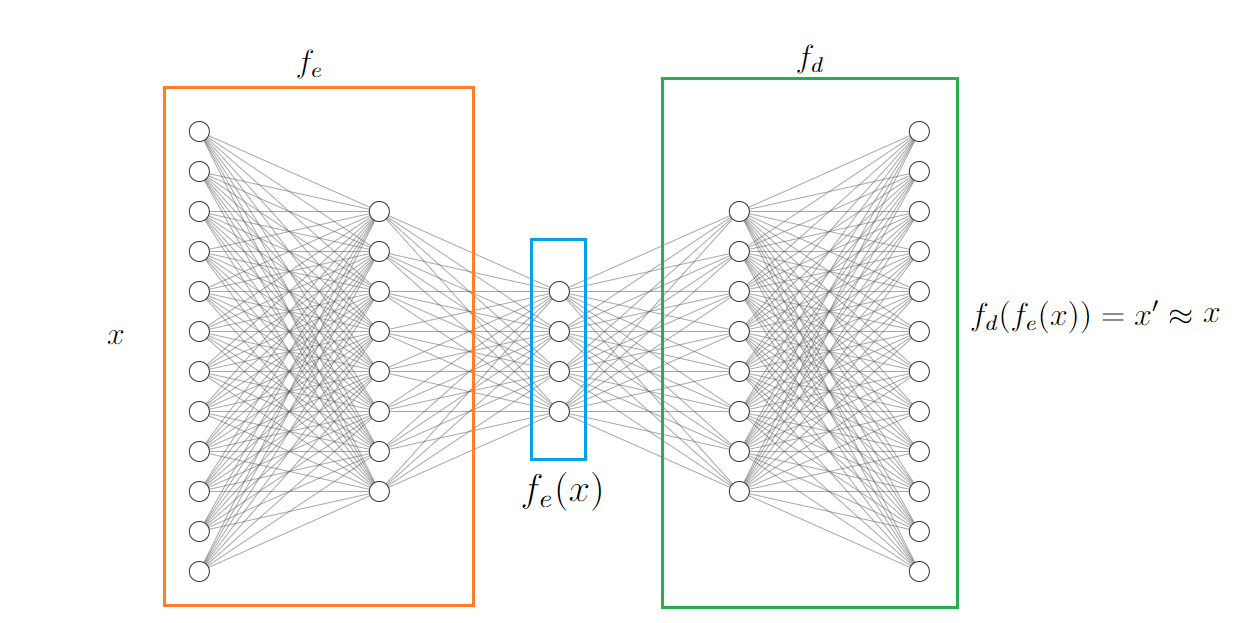
\includegraphics[width=0.9\textwidth]{imagens/p-autoencoder.png}
\caption{\label{fig:treinamentoae}Treinamento do \textit{AE}}
\end{figure}

O modelo $AE$ será treinado em $X$, e em seu espaço latente teremos uma representação do dado de entrada com a dimensionalidade reduzida, preservando suas características de maneira suficiente para que possa ser reconstruído ($x'$) ao aplicar a função de \textit{decoding}.

% ------------------------------------------------------------------------------------------
\subsection{Classificação da Intensidade}

Através do modelo de Russel sabemos que que é possível dispor as emoções em função da valência (prazer ou desprazer) e da ativação (vigor ou quietude) \cite{27}. Plutchik decompõe as emoções básicas de acordo com a intensidade, chegando a emoções compostas, formadas a partir de duas emoções com intensidades menores.

Ao longo do Capítulo \ref{Cap:Trabalhos Relacionados}, observamos trabalhos relacionados, desafios pertinentes à pesquisa e o estado da arte na área de estudo deste trabalho, que se diferencia dos pares por, além de ser um dos poucos trabalhos a lidar com o idioma português, também aborda a questão da intensidade da emoção.

Sabemos da relevância que \textit{features} espectrais carregam sobre a vocalização e vimos formas para avaliar o desempenho dos modelos. Para a etapa de classificação da intensidade, vamos construir e treinar um modelo supervisionado $j$ (e.g.: \textit{RNN}) que recebe como \textit{input} o \textit{encoding} do \textit{mel-spectrogram} dos $x_i \in X_{VIVAE_{treino}}$.

Este modelo será construído para classificar a intensidade da emoção de forma direta. Uma vez que os $x_i \in X_{VIVAE_{treino}}$ têm correspondentes em $Z$, contra domínio das intensidades, então, $j: M \rightarrow Z$, é tal que

\begin{equation}
    j(f_e(m)) = z
\end{equation}

\begin{figure}[h]
\centering
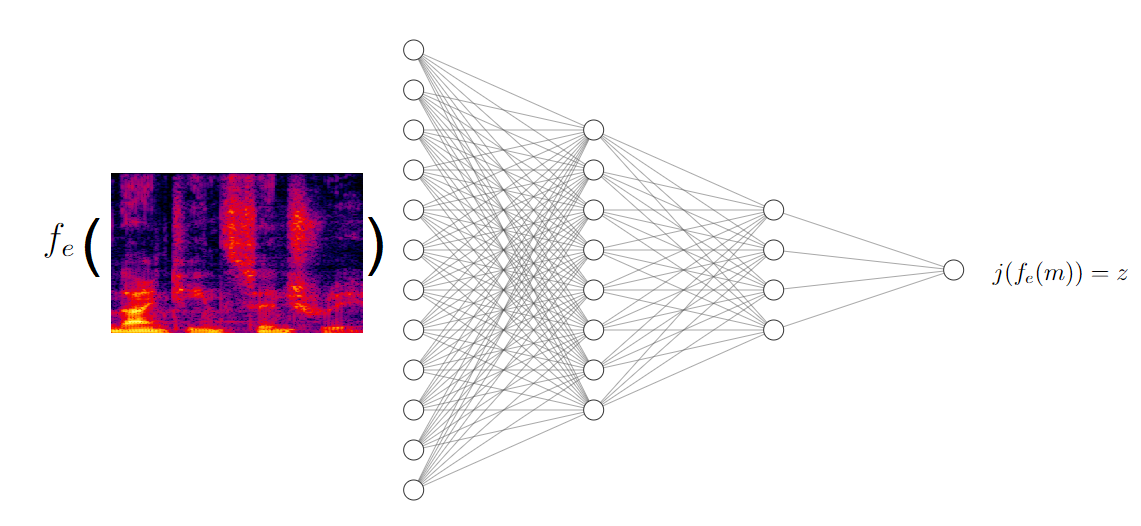
\includegraphics[width=1.0\textwidth]{imagens/p-supervisionado.png}
\caption{\label{fig:jsupervisionado}Modelo supervisionado $j$}
\end{figure}

% ------------------------------------------------------------------------------------------
\section{Validação}

Modelos de classificação (ou regressão) precisam ser validados para que possamos avaliar o seu desempenho e gerar inferências a respeito do seu comportamento. Existem diversas formas para atuar na coleta e interpretação dos seus resultados, sendo mais ou menos adequadas à natureza do modelo.%, vide as méricas expostas em \ref{sec:metricas}.

\subsubsection{Autoencoder}

Antes de seguir para a etapa de classificação (B), precisamos verificar a qualidade do modelo produzido, já que este irá prover os dados para o próximo modelo. Apesar de ser um modelo não supervisionado, podemos pensar em formas de aferir seu desempenho. Uma vez que o modelo \textit{AE} tenta reproduzir a função identidade, podemos calcular a diferença entre os atributos de entrada e os atributos de saída. Para isso, podemos utilizar o Erro Quadrático Médio (\textit{Mean Squared Error, MSE}):

\begin{equation}
    MSE = \frac{1}{n} * \sum^n_{i=1} (x_i - x'_i)^2
\end{equation}

É desejado que o \textit{MSE} para os atributos de $\{x, x'\}$ seja o mais próximo de zero, indicando que o modelo consegue reconstruir o \textit{input} com grande precisão.

Após o treinamento, vamos separar $X_{VIVAE}$ em três partes com proporções $0,8$, $0,1$ e $0,1$, que irão formar as amostras de treino ($X_{VIVAE_{treino}}$), teste ($X_{VIVAE_{teste}}$) e validação ($X_{VIVAE_{validacao}}$), respectivamente, do modelo supervisionado $j$ que iremos construir a seguir.

\subsubsection{Classificador}

Por ser tratar de um modelo supervisionado, podemos aplicar as méricas descritas em \ref{sec:metricas}, utilizando $X_{VIVAE_{validacao}}$ e $X_{VIVAE_{teste}}$ para testar e validar seus resultados. Podemos observar algumas dessas métricas na figura \ref{fig:exclassificationreport}.

\begin{figure}[h]
\centering
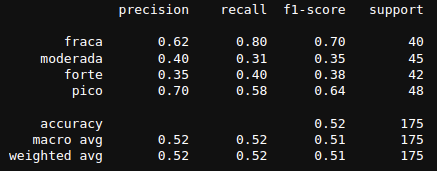
\includegraphics[width=1.0\textwidth]{imagens/ex_classification_report.png}
\caption{\label{fig:exclassificationreport}Métricas de desempenho para modelo supervisionado}
\end{figure}

Vamos assumir um limiar de 50\% para a acurácia média ponderada, análogo ao lançar de uma moeda, para considerar o modelo minimamente viável. Assim, que para cada intensidade, o modelo classifique corretamente, no mínimo, metade dos registros que pertencem àquela classe.

Uma vez que o desempenho de $j$ seja satisfatório, vamos aplicar $j$ em $X_{VERBO}$, obtendo $Z' = \{z'{_i} = j(x_i), \forall x_i \in X_{VERBO}\}$, que serão os resultados para as intensidades das emoções de $X_{VERBO}$.

\subsubsection{Aplicação em $X_{VERBO}$}

Podemos conjecturar, de forma ingênua, um limiar análogo ao do modelo supervisionado, considerando o resultado final minimamente válido caso o agrupamento dos \{u,v\} seja coerente - de acordo com os rótulos - para pelo menos 50\% dos registros de cada classe.

Como não existe correspondência entre $X_{VERBO} \rightarrow Z$, não podemos validar imediatamente as intensidades $z'$. Sabendo as intensidades reais $z_i$ dos $x_i \in X_{VIVAE}$, podemos agregar as features e intensidades, formando vetores, $v_i, u_i$, onde

\begin{itemize}
    \item $v_i = [f_e(m_i), y_i, z_i]$, onde $x_i \in X_{VIVAE}$
    \item $u_i = [f_e(m_i), y_i, j(m_i) = z'_i]$, onde $x_i \in X_{VERBO}$
\end{itemize}

Portanto, devemos ter vetores $u,v$ que contêm atributos representativos de características relativas a emoção, sua classe e a intensidade dessa emoção.

Algoritmos não supervisionados como \textit{PCA} e \textit{K-means} podem atuar como formadores de \textit{clusters} para avaliar o desempenho de geração de dados sintéticos.

Podemos então aplicar técnicas de clusterização (e.g.: \textit{PCA}) para investigar se os vetores com classe ($y$) e intensidade ($z$) são agrupáveis de forma coerente com base em suas características $y, z$ e verificar a validade de $j$ em $X_{VERBO}$.

\begin{figure}[!h]
\centering
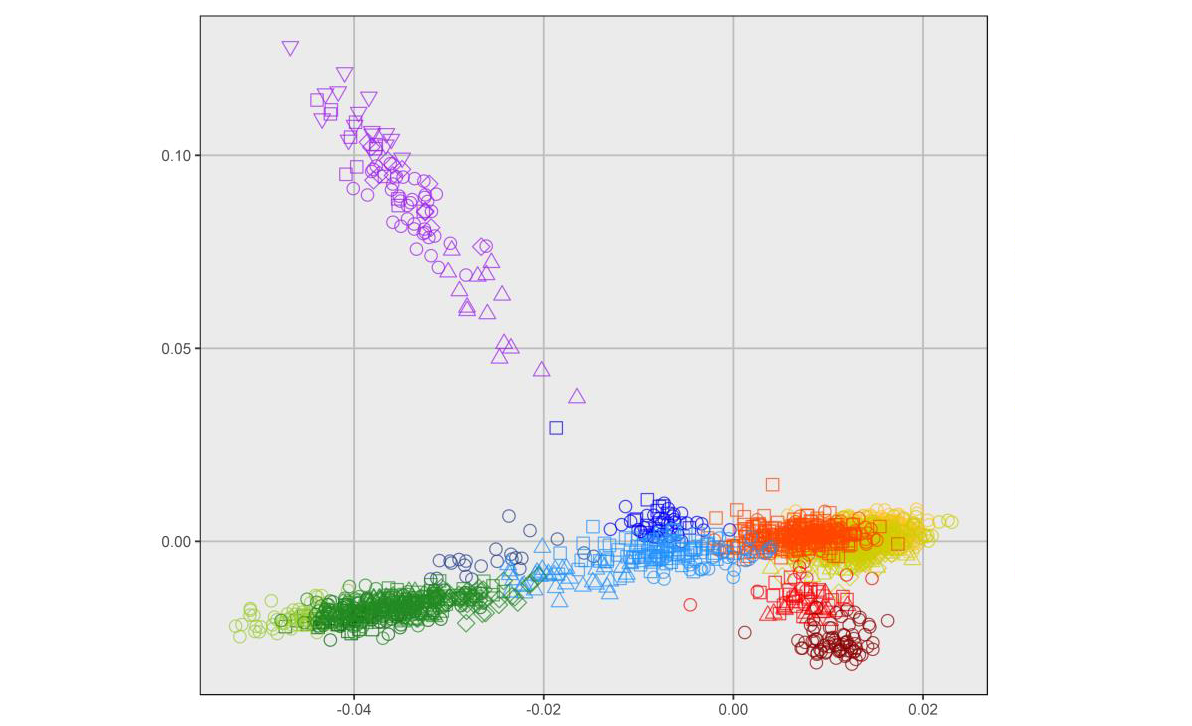
\includegraphics[width=1.0\textwidth]{imagens/p-naosupervisionado.png}
\caption{\label{fig:clusterizacaoresults}Exemplo de clusterização de resultados}
\end{figure}

% ==========================================================================================
\section{Plano de Trabalho e Cronograma}

Esta seção apresenta as atividades propostas para este projeto de pesquisa, juntamente com um cronograma de acompanhamento. Planeja-se finalizar o projeto em dois anos de atividades. Abaixo, temos enumeradas as atividades necessárias para a conclusão do Programa de Pós-Graduação em Informática da Universidade de Brasília (PPGI/UnB) e obtenção do título de Mestre. A Tabela \ref{table:cronogramaproposta} apresenta o cronograma de atividades deste plano de trabalho.\\

Atividades:

\begin{enumerate}
    \item Obtenção dos créditos obrigatórios exigidos pelo programa de mestrado;
    \item Obtenção da certificação de proficiência em idioma Inglês;
    \item Revisão da literatura, fundamentação teórica e apresentações;
    \item Redação e exame da qualificação;
    \item Planejar, realizar e analisar os experimentos;
    \item Publicação dos resultados;
    \item Redação da dissertação e defesa do mestrado.
\end{enumerate}

\begin{table}[!h]
\centering
\label{table:cronogramaproposta}
\caption{Cronograma proposto de atividades, onde \textbf{X} representa atividades finalizadas e \textbf{O} representa atividades a desenvolver}
\label{tab:my-table}
\begin{tabular}{ccccccccc}
\cline{3-9}
 & \multicolumn{1}{c|}{} & \multicolumn{7}{c|}{Atividade no trimestre} \\ \hline
\multicolumn{2}{|c|}{Período} & \multicolumn{1}{c|}{1} & \multicolumn{1}{c|}{2} & \multicolumn{1}{c|}{3} & \multicolumn{1}{c|}{4} & \multicolumn{1}{c|}{5} & \multicolumn{1}{c|}{6} & \multicolumn{1}{c|}{7} \\ \hline
\multicolumn{1}{|c|}{\multirow{2}{*}{2022}} & \multicolumn{1}{c|}{3o trimestre} & \multicolumn{1}{c|}{X} & \multicolumn{1}{c|}{} & \multicolumn{1}{c|}{} & \multicolumn{1}{c|}{} & \multicolumn{1}{c|}{} & \multicolumn{1}{c|}{} & \multicolumn{1}{c|}{} \\ \cline{2-9} 
\multicolumn{1}{|c|}{} & \multicolumn{1}{c|}{4o trimestre} & \multicolumn{1}{c|}{X} & \multicolumn{1}{c|}{X} & \multicolumn{1}{c|}{X} & \multicolumn{1}{c|}{X} & \multicolumn{1}{c|}{X} & \multicolumn{1}{c|}{} & \multicolumn{1}{c|}{} \\ \hline
\multicolumn{1}{|c|}{\multirow{4}{*}{2023}} & \multicolumn{1}{c|}{1o trimestre} & \multicolumn{1}{c|}{X} & \multicolumn{1}{c|}{} & \multicolumn{1}{c|}{O} & \multicolumn{1}{c|}{} & \multicolumn{1}{c|}{O} & \multicolumn{1}{c|}{} & \multicolumn{1}{c|}{} \\ \cline{2-9} 
\multicolumn{1}{|c|}{} & \multicolumn{1}{c|}{2o trimestre} & \multicolumn{1}{c|}{X} & \multicolumn{1}{c|}{} & \multicolumn{1}{c|}{O} & \multicolumn{1}{c|}{} & \multicolumn{1}{c|}{O} & \multicolumn{1}{c|}{} & \multicolumn{1}{c|}{} \\ \cline{2-9} 
\multicolumn{1}{|c|}{} & \multicolumn{1}{c|}{3o trimestre} & \multicolumn{1}{c|}{X} & \multicolumn{1}{c|}{} & \multicolumn{1}{c|}{O} & \multicolumn{1}{c|}{} & \multicolumn{1}{c|}{O} & \multicolumn{1}{c|}{O} & \multicolumn{1}{c|}{} \\ \cline{2-9} 
\multicolumn{1}{|c|}{} & \multicolumn{1}{c|}{4o trimestre} & \multicolumn{1}{c|}{X} & \multicolumn{1}{c|}{} & \multicolumn{1}{c|}{O} & \multicolumn{1}{c|}{} & \multicolumn{1}{c|}{O} & \multicolumn{1}{c|}{O} & \multicolumn{1}{c|}{} \\ \hline
\multicolumn{1}{|c|}{\multirow{2}{*}{2024}} & \multicolumn{1}{c|}{1o trimestre} & \multicolumn{1}{c|}{X} & \multicolumn{1}{c|}{} & \multicolumn{1}{c|}{} & \multicolumn{1}{c|}{} & \multicolumn{1}{c|}{} & \multicolumn{1}{c|}{O} & \multicolumn{1}{c|}{O} \\ \cline{2-9} 
\multicolumn{1}{|c|}{} & \multicolumn{1}{c|}{2o trimestre} & \multicolumn{1}{c|}{X} & \multicolumn{1}{c|}{} & \multicolumn{1}{c|}{} & \multicolumn{1}{c|}{} & \multicolumn{1}{c|}{} & \multicolumn{1}{c|}{O} & \multicolumn{1}{c|}{O} \\ \hline
\multicolumn{1}{l}{} & \multicolumn{1}{l}{} & \multicolumn{1}{l}{} & \multicolumn{1}{l}{} & \multicolumn{1}{l}{} & \multicolumn{1}{l}{} & \multicolumn{1}{l}{} & \multicolumn{1}{l}{} & \multicolumn{1}{l}{} \\
\multicolumn{1}{l}{} & \multicolumn{1}{l}{} & \multicolumn{1}{l}{} & \multicolumn{1}{l}{} & \multicolumn{1}{l}{} & \multicolumn{1}{l}{} & \multicolumn{1}{l}{} & \multicolumn{1}{l}{} & \multicolumn{1}{l}{}
\end{tabular}
\end{table}


% ==========================================================================================

\bibliographystyle{ieeetr}
\bibliography{100_refs}

\end{document}
